\chapter{Arrays und dynamische Programmierung}
\epigraph{If debugging is the process of removing software bugs, then programming must be the process of putting them in.}
{Edsger Dijkstra}

Bis hierhin haben wir sehr kleine Datenmengen behandelt. Unser bisheriges \enquote{Arbeitsmaterial} waren Variablen, die einige wenige Bytes halten. Eine Stärke von Computern ist es aber gerade, große Datenmengen schnell zu verarbeiten. Hier werden wir Möglichkeiten kenenn lernen, nahezu beliebig große Datenmengen im Speicher zu halten und zu manipulieren.

\section{Arrays} \label{sec:Arrays}
\emph{Arrays} (Felder) sind Gruppen von Variablen, die man sich als nummerierte Liste vorstellen kann. Die einzelnen Elemente werden über ihren \emph{Index} angesprochen, also die \enquote{Nummer der Zeile in der Liste}. Die Nummerierung beginnt hierbei \emph{bei der 0}. Alle Elemente eines Arrays haben denselben Datentyp; man sagt daher auch, das Array selbst habe einen bestimmten Datentyp.

Das Handling von Arrays geschieht über Pointer. Man speichert die Adresse des ersten Elements. Im Speicher liegen alle Werte dicht an dicht hintereinander. Um etwa das dritte Element eines Arrays anzusprechen (zu lesen oder zu überschreiben) geht man von der \emph{Startadresse} um zwei Schritte weiter. Der Abstand zur Start-Adresse wird auch \emph{Offset} genannt. Bei Arrays, deren Elemente nur ein einzelnes Byte groß sind sind also Offset und Index gleich.

\begin{tcolorbox}[title=Speicherbild]
\begin{center}
\begin{tikzpicture}
  [ 
    cell/.style={text width=8mm,
    text height=4mm, draw=black, inner sep=1mm},
    ld/.style={draw=blue,shorten >=2pt,->}
  ]
  \node (c1) at (0,0) [cell] {\ttfamily 99};
  \node (c2) at (1,0) [cell] {\ttfamily 1};
  \node (c3) at (2,0) [cell] {\ttfamily 255};
  \node (c4) at (3,0) [cell] {\ttfamily 0};
  \node (c5) at (4,0) [cell] {\ttfamily 80};
  \node (c6) at (5,0) [cell] {\ttfamily ...};

  \node (labelMem) at (7,  0) {Speicher};
  \node (labelMem) at (7,  1) {Indizes};
  \node (labelMem) at (7, -1) {Adressen};
  
  \node (a1) [below=2mm of c1]            {\tiny 0x27ff};
  \node (a2) [below=2mm of c2, color=red] {\tiny 0x2800};
  \node (a3) [below=2mm of c3]            {\tiny 0x2801};
  \node (a4) [below=2mm of c4]            {\tiny 0x2802};
  \node (a5) [below=2mm of c5]            {\tiny 0x2803};
  \node (a6) [below=2mm of c6]            {\tiny 0x2804};
  
  \node (ptr) [below=8mm of c1] {\scriptsize\ttfamily Startadresse};
  \node (vc2) [above=6mm of c1] {\scriptsize\ttfamily Index 2};
  \node (vc0) [above=2mm of c1] {\scriptsize\ttfamily Index 0};
  
  \draw [ld] (ptr.east) .. controls +(0.3,0) .. (a2.south);
  \draw [ld] (vc0.east) .. controls +(0.4,0) .. (c2.north);
  \draw [ld] (vc2.east) .. controls +(2.4,0) .. (c4.north);
\end{tikzpicture}
\end{center}
\end{tcolorbox}

\subsection{Syntax-Elemente}
Wie alle Variablen müssen auch Arrays zuerst deklariert werden. Dies geschieht in der Form:

\begin{codebox}[Syntax: Arrays deklarieren]
\begin{minted}{c}
Datentyp Name[ElementAnzahl];
\end{minted}
\end{codebox}

Damit wird ein Array vom Typ \texttt{Datentyp} angelegt, das \emph{ElementAnzahl} Elemente hat und über die Variable \texttt{Name} angesprochen werden kann. Achtung: Die Variable \texttt{Name} selbst ist vom Typ \texttt{Datentyp *}, also ein \emph{Pointer auf Daten vom Typ \texttt{Datentyp}}. Man nennt die einzelnen Elemente eines Arrays auch \emph{Instanzen von \texttt{Datentyp}}.

Wir greifen (sowohl lesend als auch schreibend) auf Arrays zu, indem wir in [eckingen Klammern] den Index des Elements schreiben, das wir ansprechen möchten (\ie seine \enquote{Nummer} in einer Liste). Man spricht von \emph{indiziertem Array-Zugriff}.

\begin{warnbox}[Indizierung ab 0]
Achtung: Indizes beginnen bei \texttt{0}. Das bedeutet, dass das letzte gültige Element des Arrays den Index \texttt{ElementAnzahl - 1} hat. Der Compiler führt bei Array-Zugriffen keine Gültigkeitskontrolle der Indizes durch. Es ist also möglich, ein Array mit 10 Elementen zu deklarieren, dann aber auf das 11. Element zuzugreifen. Wie schon in in Kapitel \ref{chp:Input} erklärt wurde, erzeugt Lese- und Schreibzugriff auf \emph{nicht-reservierte Speicherbereiche} undefiniertes Verhalten; mögliche Effekte sind Überschreiben von anderen Variablen, Programmabsturz, aber auch \enquote{nichts}, abhängig von der Struktur des Programmes. Auch, wenn ein fehlerhafter Arrayzugriff zunächst keinen Effekt hat, sollten Sie solche Speicherzugriffe dringend vermeiden, da sonst spätere Erweiterungen am Programm nicht mehr funktionieren können, obwohl diese korrekt programmiert sind.

Achten Sie daher genau auf die Codeteile, die Ihre Array-Zugriffe bestimmen.
\end{warnbox}

\begin{codebox}[Beispiel: Array-Zugriffe]
\begin{minted}[linenos]{c}
#include <stdio.h>

int main () {
   int list[100];
   
   list[42] = 666;
   
   printf("Das 43. Element der Liste 'list' ist %d.", list[42]);
}
\end{minted}
\end{codebox}

Hier wird also in Zeile 4 eine Liste angelegt, die aus 100 \mintinline{c}{int}-Werten erstellt. Wie auch sonst wird den Elementen des Arrays bei der Deklaration \emph{kein} Startwert zugewiesen -- alle 100 Elemente haben also zufällige Startwerte.

Zeile 6 greift schreibend auf das Element mit dem Index \texttt{42} zu. Da das erste Element eines Arrays den Index \texttt{0} hat, ist dies das \emph{43. Element} der Liste.

Analog dazu zeigt Zeile 8 einen lesenden Zugriff.

\begin{hintbox}[Obi-Wan-Fehler]
Der Gegensatz zwischen der menschlichen Zählweise -- beginnend bei der 1 -- und der \enquote{Computer-Zählweise} -- beginnend bei der 0 -- führt leider häufig zu \emph{Offset-Fehlern}. Tatsächlich ist der Fehlertyp, sich bei der Indexberechnung um einen Wert 1 zu irren, so häufig, dass er einen eigenen Namen hat. Aus der englischen Ausdrucksweise \emph{off by one} wurde zuerst die Kurzform \emph{OB1} und hieraus bald die Sprechweise \emph{Obi-Wan}, wie der Charakter aus Star Wars.
\end{hintbox}

Da die Array-Variable nichts weiteres als ein Pointer auf das erste Element des Arrays ist, kann auch der \emph{Dereferenzierungs-Operator} \texttt{*} benutzt werden, um das \emph{erste Element} des Arrays zu bearbeiten:

\begin{codebox}[Beispiel: Array-Zugriff mit Dereferenzierungs-Operator]
\begin{minted}[linenos]{c}
#include <stdio.h>

int main () {
   int list[100];
   
   *list = 42;
   
   printf("Das erste Element der Liste 'list' ist %d.", list[0]);
      // Ausgabe: 42
}
\end{minted}
\end{codebox}

Dieses Beispiel dient dazu, den inneren Aufbau von Arrays zu verdeutlichen. In der Praxis ist davon abzuraten, da die Verwendung des Dereferenzierungs-Operators \texttt{*} die Information \enquote{versteckt}, dass die dereferenzierte Variable mehr als ein Element hält. Benutzen Sie auch beim Zugriff auf das erste Element den Array-Index-Zugriff \texttt{[0]}.

\subsection{Initialisierung} \label{sec:arrayInit}
Wie alle Variablen werden den Elementen von Arrays bei der Deklaration keine Startwerte zugewiesen. Auch hier existiert jedoch eine Möglichkeit, bei der Deklaration eine \emph{Initialisierung} anzufügen. Dies geschieht über die Syntax:

\begin{codebox}[Syntax: Arrays deklarieren und initialisieren]
\begin{minted}{c}
Datentyp Name[ElementAnzahl] = {Wert1, ...};
\end{minted}
\end{codebox}

es wird also eine Liste der Startwerte in \{geschweifte Klammern\} gesetzt und durch Kommata voneinander getrennt. \enquote{Fehlende} Werte werden durch Nullen ergänzt. Betrachten Sie folgendes Beispiel:

\begin{codebox}[Beispiel: Arrays deklarieren und initialisieren]
\begin{minted}[linenos]{c}
#include <stdio.h>

int main () {
   int list[5] = {10, 20, 30};
   
   for (int i=0; i<5; i++) {
     printf("%d: %2d\n", i, list[i]);
  }
}
\end{minted}
\end{codebox}

\begin{cmdbox}[Ausführungseispiel: Arrays deklarieren und initialisieren]
\begin{minted}{text}
0: 10
1: 20
2: 30
3:  0
4:  0
\end{minted}
\end{cmdbox}

\begin{hintbox}[\texttt{for}-Schleifen und Array-Indizes]
\emph{Iteriert} man über die Elemente eines Arrays (\ie führt man eine Aktion mit jedem Array-Element durch), so bietet sich eine \mintinline{c}{for}-Schleife an. Die Zählvariable wird dabei mit der Zahl der Elemente verglichen. Gängig und praktisch ist der Vergleich \texttt{Zaehlvariable < ElementAnzahl}. Dies ist direkt kompatibel mit der Regel, dass der größte erlaubte Array-Index \emph{um eins kleiner} als die Zahl der Elemente ist.
\end{hintbox}

Eine solche \emph{Initializer-List} muss mindestens einen Wert enthalten. Wollen Sie also ein Array erstellen, das vollständig mit Nullen befüllt ist, so setzen Sie:

\begin{codebox}[Syntax: Arrays deklarieren und null-initialisieren]
\begin{minted}{c}
Datentyp Name[ElementAnzahl] = {0};
\end{minted}
\end{codebox}

\begin{plusbox}[C++: leere \emph{Initializer-List}]
In der Sprache C++ ist es erlaubt, eine leere Liste zu übergeben um das Array mit null-Werten zu initialisieren:

\vspace{5pt}
\begin{codebox}[C++-Syntax: Arrays deklarieren und null-initialisieren]
\begin{minted}{c}
Datatype Name[ElementCount] = {};
\end{minted}
\end{codebox}

Dies hat dort jedoch untergeordnete Bedeutung, da die Sprache C++ Konzepte anbietet, die C-Arrays ersetzen und diesen vorzuziehen sind. Als Stichworte seien genannt:
\begin{itemize}
\item \mintinline{c++}{std::array}  (\url{https://en.cppreference.com/w/cpp/container/array})
\item \mintinline{c++}{std::vector} (\url{https://en.cppreference.com/w/cpp/container/vector})
\item \mintinline{c++}{std::list}   (\url{https://en.cppreference.com/w/cpp/container/list})
\item \mintinline{c++}{std::map}    (\url{https://en.cppreference.com/w/cpp/container/map})
\end{itemize}
\end{plusbox}

Bei der Verwendung von \emph{Initializer-Lists} ist es auch möglich, die Anzahl der Listenelemente bei der Deklaration auszulassen. Der Compiler erstellt dann ein Array, das genau groß genug ist, um alle Werte in der \emph{Initializer-List} zu fassen. Die Deklaration des Arrays geschieht dann mit leeren eckigen Klammern []:

\begin{codebox}[Syntax: Arrays-Deklaration mit automatischer Bestimmung der Array-Größe]
\begin{minted}{c}
Datentyp Name[] = {Wert1, ...};
\end{minted}
\end{codebox}

\begin{codebox}[Beispiel: Array mit 3 Elementen ohne explizite Bestimmung der Arraygröße]
\begin{minted}[linenos]{c}
int list[] = {1, 2, 3};
\end{minted}
\end{codebox}

In Abschnitt \ref{sec:sizeof} werden wir eine Möglichkeit kennen lernen, zur \emph{Laufzeit} die Größe eines solchen Arrays zu ermitteln.

\subsection{Pointer-Arithmetik}
Arrays werden über Pointer angesprochen. Pointer sind Ganzzahl-Werte, mit denen gerechnet werden kann. Rechnungen mit Pointer-Variablen verhalten sich aber anders als mit normalen Variablen.

Bei der Addition und Subtraktion wird der Datentyp der Pointer-Variable mit einbezogen: Der addierte Wert wird vor der Addition mit der Registerbreite des Pointer-Grundtyps multipliziert. Betrachten Sie das folgende Beispiel:

\begin{codebox}[Beispiel: Pointer-Arithmetik]
\begin{minted}[linenos]{c}
#include <stdio.h>

int main () {
   int list[100];
   
   list[0] = 1;
   list[1] = 2;
   
   printf("start point: %p\n", list    );
   printf("plus one:    %p\n", list + 1);
   
   printf("at start:     %d\n", * list     );
   printf("at plus one:  %d\n", *(list + 1));
   printf("at index one: %d\n",   list  [1]);
}
\end{minted}
\end{codebox}

\begin{cmdbox}[Ausgabebeispiel: Pointer-Arithmetik]
\begin{minted}{text}
start point: 0x7ffcf4413c30
plus one:    0x7ffcf4413c34
at start:     1
at plus one:  2
at index one: 2
\end{minted}
\end{cmdbox}

Wir lassen uns die Pointer \texttt{list} und \texttt{list + 1} ausgeben. Obwohl die Konstante \texttt{1} addiert wird, unterscheiden sich die Ausgaben um den Wert \texttt{4} -- der Register-Breite einer \mintinline{c}{int}-Variablen. Ändern wir das Beispiel so ab, dass \texttt{list} ein \mintinline{c}{double}-Array wird, so finden wir einen Unterschied von \texttt{8}. Die Addition geht also um \enquote{ganze Speicherstellen} oder \enquote{ganze Feld-Elemente} weiter, statt um einzelne Bytes.

Dies beeinflusst selbstverständlich auch die \emph{Dereferenzierung}. Damit verhält sich die Dereferenzierung eines Pointers nach Addition genauso wie der Index-Zugriffs-Operator \texttt{[]}. Entsprechend ist die Ausgabe von Zeile 13 und Zeile 14 identisch.

Die Subtraktion verhält sich analog -- auch hier ändert sich die Adresse, auf die der Pointer zeigt nur um \enquote{ganze Speicherstellen}. Multiplikation, Division oder andere Operationen sind mit Pointer-Variablen nicht möglich.

\subsection{Mehrdimensionale Arrays} \label{sec:MultiDimArray}
Wir haben Arrays bislang als eindimensionale Listen kennen gelernt, die im Speicher dicht an dicht gepackt sind. Es ist aber auch möglich, zweidimensionale Tabellen oder höherdimensionale Objekte abzubilden. Betrachten wir das Beispiel einer (zweidimensionalen) Tabelle:

\begin{tcolorbox}
	[title=Speicherbild einer Tabelle,
	 arc=0pt,
	 outer arc=0pt
	]
\begin{center}
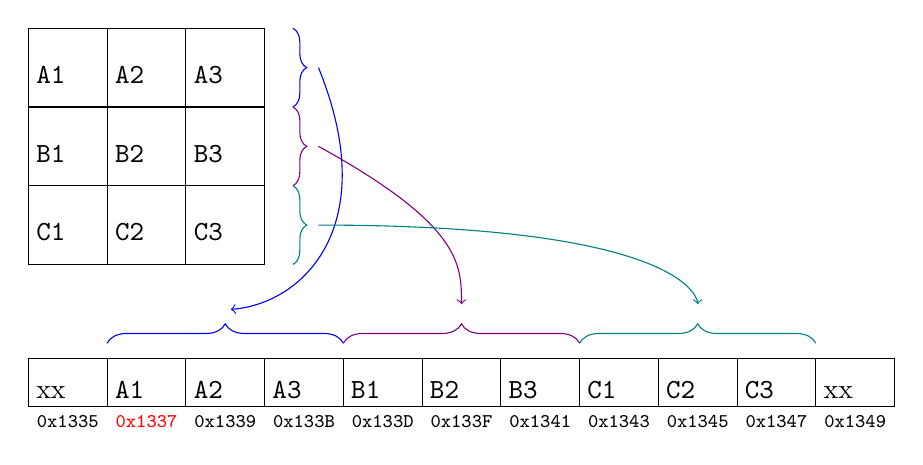
\begin{tikzpicture}
[ 
    cell/.style={text width=8mm,
    text height=4mm, draw=black, inner sep=1mm},
    ld/.style={draw=blue,shorten >=2pt,->},
    flow/.style={draw=black,->,shorten >=2pt}
]  
  \node [draw,minimum height=1cm] (cA1) at (0, 5) [cell] {\texttt{A1}};
  \node [draw,minimum height=1cm] (cA2) at (1, 5) [cell] {\texttt{A2}};
  \node [draw,minimum height=1cm] (cA3) at (2, 5) [cell] {\texttt{A3}};
  
  \node [draw,minimum height=1cm] (cB1) at (0, 4) [cell] {\texttt{B1}};
  \node [draw,minimum height=1cm] (cB2) at (1, 4) [cell] {\texttt{B2}};
  \node [draw,minimum height=1cm] (cB3) at (2, 4) [cell] {\texttt{B3}};
  
  \node [draw,minimum height=1cm] (cC1) at (0, 3) [cell] {\texttt{C1}};
  \node [draw,minimum height=1cm] (cC2) at (1, 3) [cell] {\texttt{C2}};
  \node [draw,minimum height=1cm] (cC3) at (2, 3) [cell] {\texttt{C3}};
  
  \node (m0) at (0, 1) [cell] {xx};
  
  \node (m1) at (1, 1) [cell] {\texttt{A1}};
  \node (m2) at (2, 1) [cell] {\texttt{A2}};
  \node (m3) at (3, 1) [cell] {\texttt{A3}};
  \node (m4) at (4, 1) [cell] {\texttt{B1}};
  \node (m5) at (5, 1) [cell] {\texttt{B2}};
  \node (m6) at (6, 1) [cell] {\texttt{B3}};
  \node (m7) at (7, 1) [cell] {\texttt{C1}};
  \node (m8) at (8, 1) [cell] {\texttt{C2}};
  \node (m9) at (9, 1) [cell] {\texttt{C3}};

  \node (mx) at (10, 1) [cell] {xx};
  
  \draw [decorate, decoration={brace, amplitude=5pt, mirror}, xshift=-4pt, yshift=0pt, blue]
  		(3.0, 4.5) -- (3.0, 5.5) 
  		node [midway, xshift=+0.2cm]
		(lA) {};
  \draw [decorate, decoration={brace, amplitude=5pt, mirror}, xshift=-4pt, yshift=0pt, violet]
  		(3.0, 3.5) -- (3.0, 4.5) 
  		node [midway, xshift=+0.2cm]
		(lB) {};
  \draw [decorate, decoration={brace, amplitude=5pt, mirror}, xshift=-4pt, yshift=0pt, teal]
  		(3.0, 2.5) -- (3.0, 3.5) 
  		node [midway, xshift=+0.2cm]
		(lC) {};
  
  \draw [decorate, decoration={brace,amplitude=7pt}, xshift=-0pt, yshift=0pt, blue]
  		(0.5, 1.5) -- (3.5, 1.5) node [black, midway, yshift=+0.3cm] 
		(mA) {};
  \draw [decorate, decoration={brace,amplitude=7pt}, xshift=-0pt, yshift=0pt, violet]
  		(3.5, 1.5) -- (6.5, 1.5) node [black, midway, yshift=+0.3cm] 
		(mB) {};
  \draw [decorate, decoration={brace,amplitude=7pt}, xshift=-0pt, yshift=0pt, teal]
  		(6.5, 1.5) -- (9.5, 1.5) node [black, midway, yshift=+0.3cm] 
		(mC) {};
  
  \draw[flow, blue]   (lA.east) .. controls (4, 3) and (3, 2.0) .. (mA.north);
  \draw[flow, violet] (lB.east) .. controls (5, 3) and (5, 2.5) .. (mB.north);
  \draw[flow, teal]   (lC.east) .. controls (8, 3) and (8, 2.0) .. (mC.north);
  
  \node (a0) at (0, 0.5)       {\scriptsize\texttt{0x1335}};
  
  \node (a1) at (1, 0.5) [red] {\scriptsize\texttt{0x1337}};
  \node (a2) at (2, 0.5)       {\scriptsize\texttt{0x1339}};
  \node (a3) at (3, 0.5)       {\scriptsize\texttt{0x133B}};
  \node (a4) at (4, 0.5)       {\scriptsize\texttt{0x133D}};
  \node (a5) at (5, 0.5)       {\scriptsize\texttt{0x133F}};
  \node (a6) at (6, 0.5)       {\scriptsize\texttt{0x1341}};
  \node (a7) at (7, 0.5)       {\scriptsize\texttt{0x1343}};
  \node (a8) at (8, 0.5)       {\scriptsize\texttt{0x1345}};
  \node (a9) at (9, 0.5)       {\scriptsize\texttt{0x1347}};
  
  \node (a0) at (10, 0.5)      {\scriptsize\texttt{0x1349}};
\end{tikzpicture}
\end{center}
\end{tcolorbox}

Tabellen können im Speicher \enquote{geplättet} als Kette abgelegt werden. Jede Zeile der Tabelle -- für sich eine Liste -- fügt sich im Speicher an die nächste. Eine zweidimensionale Tabelle kann also als \enquote{Liste von Listen} gesehen werden.

Jede Zelle der Tabelle hat eine Zeilen- und Spaltennummer. Wir wissen, dass die Tabelle 3 Spalten breit ist. Damit finden wir für den Index in der \enquote{geplätteten Liste}:
\begin{center}
\texttt{Index = (Breite * Zeile) + Spalte}
\end{center}
wobei die Zählung von Zeile und Spalte bei 0 beginnt.

Umgekehrt kann aus der Position einer Zelle in der geplätteten Liste wieder die Koordinate in der Tabelle berechnet werden: Die Zelle mit dem Wert \texttt{B2} ist die fünfte Zelle der \enquote{geplätteten Liste} im Speicher und hat damit den Index 4. Wir wissen, dass unsere Tabelle eine Breite von 3 Zellen hatte. Mit diesen Informationen können wir ansetzen:
\begin{center}
\texttt{ Zeile = Index / Breite}\\
\texttt{Spalte = Index \% Breite}
\end{center}

Der Compiler kann solche Strukturen automatisch anlegen. Bei der Deklaration eines mehrdimensionalen Arrays hängen wir für jede Dimension eine eigene [Klammer] an. Ebenso wird beim (lesenden wie schreibenden) Zugriff jede Dimension durch eine eigene Klammer referenziert.

\begin{codebox}[Syntax: Arrays-Deklaration mehrdimensionaler Arrays]
\begin{minted}{c}
Datentyp Name[dim1][dim2][...];
\end{minted}
\end{codebox}

\begin{codebox}[Syntax: Zugriff auf mehrdimensionale Arrays]
\begin{minted}{c}
Name[Index1][Index2][...] = ...;
\end{minted}
\end{codebox}

Im Falle einer Tabelle könnte \texttt{dim1} dann für die Anzahl der Zeilen und \texttt{dim2} für die Anzahl der Spalten der Tabelle stehen.

Mehrdimensionale Arrays können auch direkt bei der Deklaration Initialisiert werden. Hierzu werden verschachtelte \{geschweifte Klammern\} benutzt. Betrachten Sie das folgende Beispiel:

\begin{codebox}[Beispiel: Tabelle als mehrdimensionales C-Array]
\begin{minted}[linenos]{c}
#include <stdio.h>

int main () {
   int table[3][4] = {
      {1, 2, 3, - 6},
      {4, 5, 6, -15},
      {7, 8, 9, -24}
   };
   
   for    (int row = 0; row < 3; row ++) {
      for (int col = 0; col < 4; col ++) {
         printf("%d\t", table[row][col]);
     }
         printf("\n");
   }
   
   printf("\n");
   table[0][1] = 0;
   
   for    (int row = 0; row < 3; row ++) {
      for (int col = 0; col < 4; col ++) {
         printf("%d\t", table[row][col]);
     }
         printf("\n");
   }
}
\end{minted}
\end{codebox}

\begin{cmdbox}[Ausführungseispiel: Tabelle als mehrdimensionales C-Array]
\begin{minted}{text}
1       2       3       -6
4       5       6       -15
7       8       9       -24

1       0       3       -6
4       5       6       -15
7       8       9       -24
\end{minted}
\end{cmdbox}

In den Zeilen 4..8 definieren wir eine Tabelle mit 3 Zeilen und 4 Spalten (auch als \emph{3x4-Matrix} bezeichnet). Und befüllen diese direkt mit Werten. 

Wir können \texttt{table[0]} als \enquote{die erste Zeile der Tabelle} lesen. Dieses Objekt ist selbst eine Liste von vier Zahlen. Entsprechend wird dem Objekt \texttt{table[0]} die Liste \texttt{\{1, 2, 3, -6\}} zugewiesen. Analog funktioniert die Zuweisung der nächsten zwei Zeilen.

Mit \texttt{printf} geben wir in Zeile 12 das Tabellenelement in der Zeile \texttt{row} und der Spalte \texttt{col} aus. Diese Variablen werden im Kontext von \mintinline{c}{for}-Schleifen deklariert und mit Werten befüllt.

In Zeile 18 ändern Wir Zeile 1, Spalte 2 auf den Wert \texttt{0} und geben die veränderte Tabelle dann nochmals aus.

\begin{warnbox}[Reihenfolge der Dimensionen]
Achten Sie bei mehrdimensionalen Arrays auch auf die Reihenfolge der Indizes. Eine Vertauschung kann zu Zugriffen außerhalb Ihrer Tabelle führen und bewirkt ebenfalls wieder undefiniertes Verhalten!

Wenn Sie im oberen Beispiel die Zeile
\begin{center}
\mintinline{c}{printf("%d\n", table[3][2]);}
\end{center}
anfügen, so geschieht folgendes:

Der Compiler versucht auf Zeile 4, Spalte 3 zuzugreifen. Nach der zuvor gezeigten Formel wird berechnet:
\begin{center}
\texttt{Index = (Breite * Zeile) + Spalte = (4 * 3) + 2 = 14}
\end{center}
Unsere Tabelle hat aber nur insgesamt 12 Werte. Der Zugriff führt also auf einen nicht-reservierten Speicherbereich und liefert eine \enquote{unsinnige} Ausgabe.
\end{warnbox}

\section{Dynamische Speicherverwaltung} \label{sec:dynArrays}
Die bisher gezeigten Techniken funktionieren, solange zur \emph{Compile-Zeit} bereits bekannt ist, mit wie vielen Elementen gearbeitet werden soll\footnote{Oder, wenn eine Maximalzahl von Elementen bekannt ist, die höchstes auftreten können. Man benutzt dann ein Array dieser Maximalgröße und befüllt nur so viele Einträge, wie tatsächlich Daten anfallen.}. Häufig steht aber erst zur \emph{Laufzeit} fest, wie viele Daten tatsächlich anfallen. Hier wollen wir Techniken \emph{dynamischer Speicherverwaltung} kennenlernen. \ie \enquote{im laufenden Betrieb} Felder erstellen, vergrößern und verkleinern und diese Operationen direkt von Usereingaben abhängig machen.

\subsection{Speicher allozieren und freigeben: \texttt{malloc}, \texttt{calloc} und \texttt{free}}
\label{sec:allocation}
Wir haben im vorigen Abschnitt \ref{sec:Arrays} kennen gelernt, wie wir mit einem Pointer auf Feldelemente zugreifen. Für die dynamische Speicherverwaltung benötigen wir also lediglich ein Mittel, einen Pointer auf einen geeignet großen Speicherbereich zu bekommen. Dazu dienen die Befehle \texttt{malloc} und \texttt{calloc}, die über den header \texttt{stdlib.h} eingebunden werden können.

Beide Befehle \emph{allozieren} einen Speicherbereich (\ie stellen eine Anfrage ans Betriebssystem, Speicher für die ausschließliche Verwendung durch das allozierende Programm zu reservieren) und geben einen Pointer auf den Beginn dieses Speicherbereichs zurück. Der Befehl \texttt{calloc} initialisiert diesen Speicherbereich zusätzlich mit Nullen. Der Befehl \texttt{malloc} arbeitet schneller, da das auf-null-Setzen entfallen kann. Die Abkürzungen stehen also für \emph{memory allocate} und \emph{clear allocate}.

Die Syntax der beiden Befehle ist ähnlich, leider aber nicht identisch:
\begin{tcbraster}[raster columns=2,
                  raster equal height,
                  nobeforeafter,
                  raster column skip=0.5cm]
\begin{codebox}[Syntax: \texttt{malloc}]
\begin{minted}{c}
pointer = malloc(AnzahlBytes);
\end{minted}
\end{codebox}
%
\begin{codebox}[Syntax: \texttt{calloc}]
\begin{minted}{c}
pointer = calloc(AnzahlFelder, 
                 BytesProFeld);
\end{minted}
\end{codebox}
\end{tcbraster}

Hierbei ist \texttt{AnzahlBytes} eine vorzeichenlose (\ie positive) Ganzzahl, die angibt, wie viele Bytes im Speicher benötigt werden. Ähnlich beschreibt \texttt{AnzahlFelder} eine vorzeichenlose Ganzzahl, die die Zahl der \emph{Elemente} angibt, für die Speicher alloziert werden soll. \texttt{BytesProFeld} ist dann die Größe \emph{eines} Elements in Bytes.

Auf die Elemente des so reservierten Speicherbereichs kann über dieselben Syntaxelemente zugegriffen werden, die wir schon aus Abschnitt \ref{sec:Arrays} kennen. Selbstverständlich müssen wir auch hier die selbe Sorgfalt bei der Berechnung der Indizes anlegen.

Reservierte Speicherbereiche sollten nach Nutzung wieder freigegeben werden\footnote{moderne Betriebssysteme geben bei Beenden eines Programms allen von diesem allozierten Speicher automatisch wieder frei, auch wenn dieser nicht vom Programmierer freigegeben wurde. Dieses Verhalten kann aber insbesondere für Elektronik-Anwendungen nicht garantiert werden. Allgemein gilt es als \emph{guter Stil}, zu jeder Zeit nur soviel Speicher zu beanspruchen, wie tatsächlich benötigt wird.}. Dazu dient der Befehl \texttt{free}, der ebenfalls mit dem Header \texttt{stdlib.h} eingebunden wird. Die Syntax ist denkbar einfach:

\begin{codebox}[Syntax: \texttt{free}]
\begin{minted}{c}
free(pointer);
\end{minted}
\end{codebox}

Wird reservierter Speicher nicht mehr freigeben, so steht dieser anderen Prozessen nicht zur Verfügung. Programme laufen langsamer und können potentiell Aufgaben nicht mehr bewältigen, da die notwendige Speicherkapazität \enquote{nicht zur Verfügung steht}. Man spricht von \emph{memory leakage}.

Damit können wir das folgende Beispiel verstehen:

\begin{codebox}[Beispiel: Dynamische Speicherverwaltung]
\begin{minted}[linenos]{c}
#include <stdio.h>
#include <stdlib.h>

int main () {
  double * array = malloc(88);      // 1 double = 8 byte ==> 11 Speicherstellen
  double * nulls = calloc(11, 8);   // dito
  int i;
  
  for (i=0; i<11; i++) {
     array[i] = (i * i) / 100.0;
     printf("%2d    malloc: %4.2lf   calloc: %4.2lf\n", i, array[i], nulls[i]);
  }
  
  free(array);
  free(nulls);
}
\end{minted}
\end{codebox}

\begin{cmdbox}[Ausfphrungsbeispiel: Dynamische Speicherverwaltung]
\begin{minted}{text}
 0    malloc: 0.00   calloc: 0.00
 1    malloc: 0.01   calloc: 0.00
 2    malloc: 0.04   calloc: 0.00
 3    malloc: 0.09   calloc: 0.00
 4    malloc: 0.16   calloc: 0.00
 5    malloc: 0.25   calloc: 0.00
 6    malloc: 0.36   calloc: 0.00
 7    malloc: 0.49   calloc: 0.00
 8    malloc: 0.64   calloc: 0.00
 9    malloc: 0.81   calloc: 0.00
10    malloc: 1.00   calloc: 0.00
\end{minted}
\end{cmdbox}

\begin{hintbox}[Datentypen und dynamische Speicherverwaltung]
Wir hatten bereits angesprochen, dass bei der Arbeit in der Sprache C besonderer Wert auf die Verwendung der korrekten Datentypen zu legen ist. Daher auch einige Kommentare zu diesem Thema:

Die Parameter \texttt{AnzahlBytes}, \texttt{AnzahlFelder} und \texttt{BytesProFeld} sind formell vom Typ \texttt{size\_t}. Dieser wird im Header \texttt{stdlib.h} definiert und ist \idR ein \mintinline{c}{unsigned long int}, in jedem Fall aber ein vorzeichenloser Ganzzahl-Typ. Im Falle des \texttt{gcc} wird ein \mintinline{c}{unsigned long int} verwendet.

Der Rückgabewert von \texttt{calloc} und \texttt{malloc} ist ein \mintinline{c}{void *}, also ein Pointer auf einen unspezifizierten Datentyp. Dies macht die Verwendung von \texttt{malloc} und \texttt{calloc} mit Pointern jeden beliebigen Typs möglich.
\end{hintbox}

\begin{warnbox}[Zugriffe nach \texttt{free}]
Auf Felder, die bereits mit \texttt{free} freigegeben werden, darf nicht mehr zugegriffen werden. Das bedeutet, dass weder Lesen (mit dem Dereferenzierungs-Operator \texttt{*} oder dem Array-Zugriffsoperator \texttt{[]}) noch Schreiben (mit denselben Operatoren) und insbesondere keine \enquote{zweite Freigabe} mit \texttt{free} stattfinden darf. Beim Lesen und Schreiben ist das Verhalten undefiniert; bei \texttt{free} stürzt das Programm ab.
\end{warnbox}

\begin{hintbox}[Praxistipp: \texttt{alloc}s und \texttt{free} gleichzeitig schreiben]
Um in komplexeren Aufgaben nicht zu vergessen, ein Feld freizugeben, habe ich mir angewohnt, direkt nach \texttt{malloc} bzw. \texttt{calloc} ein zugehöriges \texttt{free} zu tippen. Erst danach schreibe ich den Code, der den so reservierten und wieder freigegebenen Speicherbereich auch tatsächlich nutzt.
\end{hintbox}

\begin{hintbox}[Sinnvolle und einheitliche Programmlogik]
Obwohl \texttt{malloc} und \texttt{calloc} dieselbe Kernaufgabe erfüllen -- das Allozieren von Speicher -- unterscheiden sie sich in ihrer Anwendung. Bei \texttt{malloc} wird die benötigte \emph{Speichergröße} angegeben, während \texttt{calloc} als Parameter die \emph{Feldzahl} und \emph{Feldgröße} erwartet. Dieser Unterschied macht das Arbeiten unangenehm, da man als ProgrammierIn auswendig behalten muss, welcher der sehr ähnlichen Befehle nun welche Form erwartet.

Leider ist es nicht mehr möglich, einen der beiden Befehle in einer neuen Version der Sprache C so zu ändern, dass beide derselben Syntax folgen, da sonst viele ältere Programmcodes nicht mehr mit dem neuen Compiler \emph{kompatibel} sind. Solche \emph{legacy issues} ziehen sich durch die Welt der Informatik und bereiten an verschiedensten Stellen Schwierigkeiten. Einmal etabliert lassen sich auch ungünstige Standards aber nicht mehr loswerden, wie auch Abbildung \ref{fig:xkcd-standards} illustriert.

Mit Blick auf dieses Negativ-Beispiel will ich Sie dazu aufrufen, sich eine einheitliche Struktur und Logik für Ihr Projekt zu überlegen, \emph{bevor Sie die erste Codezeile schreiben}. Wir werden insbesondere in Kapitel \ref{chp:funcs} auf Möglichkeiten stoßen, die solche Überlegungen erfordern.
\end{hintbox}

\begin{hintbox}[Feldgrößen ermitteln mit \texttt{sizeof}]
C stellt eine Vielzahl von Datentypen bereit, die jeweils andere Speicherbedarfe haben. Anstatt alle diese auswendig zu lernen sollte man mit der Funktion \mintinline{c}{sizeof} arbeiten, die die Registerbreite jedes beliebigen Typs in Bytes zurück gibt. Im obigen Beispiel können wir damit auch schreiben:
\begin{codebox}[Beispiel: Dynamische Speicherverwaltung und \texttt{sizeof}]
\begin{minted}[linenos, firstnumber=5]{c}
double * array = malloc(11 * sizeof(double));
double * nulls = calloc(11,  sizeof(double));
\end{minted}
\end{codebox}
In Abschnitt \ref{sec:sizeof} erfahren Sie mehr zu diesem Operator.
\end{hintbox}

\begin{figure}
\begin{center}
\includegraphics[width=.8\linewidth]{./gfx/xkcd-standards}
\caption
[Langlebigkeit von Standards in der IT]
{Langlebigkeit von Standards in der IT. Quelle: \url{https://xkcd.com/927/}} \label{fig:xkcd-standards}
\end{center}
\end{figure}

\begin{warnbox}[Erfolg der Allozierung prüfen]
In seltenen Fällen kann die Allozierung von Speicher fehlschlagen. Dies ist insbesondere dann der Fall, wenn nicht mehr ausreichend \emph{zusammenhängender} Speicher zur Verfügung steht, um ein Array der gewünschten Größe darin unterzubringen. In diesem Fall ist der Rückgabewert von \texttt{calloc} und \texttt{malloc} ein Null-Pointer (\ie der Wert \texttt{0}). Auf die Adresse \texttt{0} darf nicht zugegriffen werden; jeder Zugriff führt zum Programmabsturz. Daher sollte nach jedem \texttt{alloc}-Befehl eine Fehlerprüfung stattfinden. Mit dem Befehl \texttt{exit} aus der \texttt{stdlib.h} können wir etwa das Programm beenden. In Kapitel \ref{chp:OS-Link} werden wir hierzu mehr hören.

\begin{codebox}[Beispiel: Fehlerprüfung nachg Allozierung]
\begin{minted}[linenos]{c}
int * array = malloc(20);
if (!array) {
   printf("Fehler! Speicher konnte nicht alloziert werden!\n");
   exit(-1); // Programm beenden.
}
\end{minted}
\end{codebox}
\end{warnbox}

\subsection{Feldgrößen ändern: \texttt{realloc}} \label{sec:realloc}
Der Befehl \texttt{realloc} (eingebunden über den Header \texttt{stdlib.h}) ändert die Größe eines bestehenden Arrays und erhält alle Werte bei (sofern sie in noch \enquote{in das neue Array passen}). In der Regel ändert sich der Wert des Pointers auf den Beginn des Arrays nicht. Bei Vergrößerung kann es jedoch sein, dass das Array sonst mit einem anderen reservierten Speicherbereich (\eg ein anderes Array) überlappt. In diesem Fall wird \texttt{realloc} das gesamte Array an eine neue Stelle kopieren.

\begin{tcolorbox}[title=Visualisierung: Arraygrößen ändern]
Betrachten wir zuerst den Fall, in dem sich zwischen dem Ende eines zu vergrößernden Arrays und dem nächsten reservierten Speicherbereich viel Platz befindet. \texttt{realloc} wird lediglich zusätzlichen Platz reservieren und sonst keine Änderungen vornehmen.

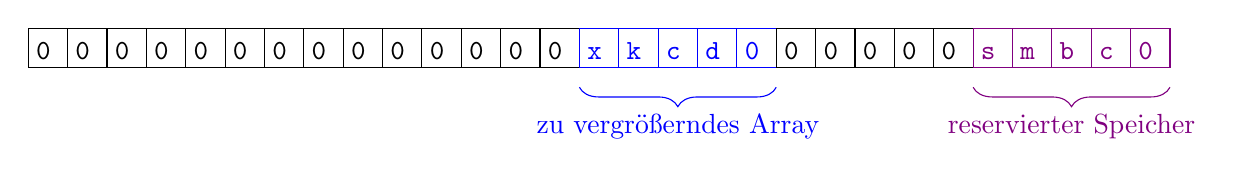
\begin{tikzpicture}
  [ 
    cell/.style={
       text width =3mm,
       text height=3mm, 
       draw=black, 
       inner sep=1mm
    },
    ld/.style={
       draw=blue,
       shorten >=2pt,
       ->
    }
  ]
  \node (c00) at ( 0.0,1) [cell]         {\ttfamily 0};
  \node (c01) at ( 0.5,1) [cell]         {\ttfamily 0};
  \node (c02) at ( 1.0,1) [cell]         {\ttfamily 0};
  \node (c03) at ( 1.5,1) [cell]         {\ttfamily 0};
  \node (c04) at ( 2.0,1) [cell]         {\ttfamily 0};
  \node (c05) at ( 2.5,1) [cell]         {\ttfamily 0};
  \node (c06) at ( 3.0,1) [cell]         {\ttfamily 0};
  \node (c07) at ( 3.5,1) [cell]         {\ttfamily 0};
  \node (c08) at ( 4.0,1) [cell]         {\ttfamily 0};
  \node (c09) at ( 4.5,1) [cell]         {\ttfamily 0};
  \node (c10) at ( 5.0,1) [cell]         {\ttfamily 0};
  \node (c11) at ( 5.5,1) [cell]         {\ttfamily 0};
  \node (c12) at ( 6.0,1) [cell]         {\ttfamily 0};
  \node (c13) at ( 6.5,1) [cell]         {\ttfamily 0};
  \node (c14) at ( 7.0,1) [cell, blue]   {\ttfamily x};
  \node (c15) at ( 7.5,1) [cell, blue]   {\ttfamily k};
  \node (c16) at ( 8.0,1) [cell, blue]   {\ttfamily c};
  \node (c17) at ( 8.5,1) [cell, blue]   {\ttfamily d};
  \node (c18) at ( 9.0,1) [cell, blue]   {\ttfamily 0};
  \node (c19) at ( 9.5,1) [cell]         {\ttfamily 0};
  \node (c20) at (10.0,1) [cell]         {\ttfamily 0};
  \node (c21) at (10.5,1) [cell]         {\ttfamily 0};
  \node (c22) at (11.0,1) [cell]         {\ttfamily 0};
  \node (c23) at (11.5,1) [cell]         {\ttfamily 0};
  \node (c24) at (12.0,1) [cell, violet] {\ttfamily s};
  \node (c25) at (12.5,1) [cell, violet] {\ttfamily m};
  \node (c26) at (13.0,1) [cell, violet] {\ttfamily b};
  \node (c27) at (13.5,1) [cell, violet] {\ttfamily c};
  \node (c28) at (14.0,1) [cell, violet] {\ttfamily 0};
  
  \draw [decorate, decoration={brace,amplitude=7pt, mirror}, xshift=-0pt, yshift=0pt, blue]
  		( 6.75, 0.5) -- ( 9.25, 0.5) node [blue, midway, yshift=-0.5cm] 
		(braceArrayPreResize) {zu vergrößerndes Array};

  \draw [decorate, decoration={brace,amplitude=7pt, mirror}, xshift=-0pt, yshift=0pt, violet]
  		(11.75, 0.5) -- (14.25, 0.5) node [violet, midway, yshift=-0.5cm] 
		(braceArrayPreResize) {reservierter Speicher};
\end{tikzpicture}

Soll nun das Array um drei Zellen vergrößert werden, so wird es einfach \enquote{nach hinten verlängert}:

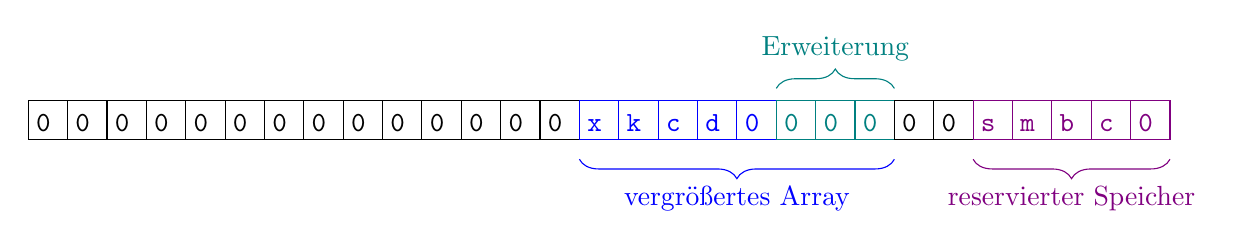
\begin{tikzpicture}
  [ 
    cell/.style={
       text width =3mm,
       text height=3mm, 
       draw=black, 
       inner sep=1mm
    },
    ld/.style={
       draw=blue,
       shorten >=2pt,
       ->
    }
  ]
  \node (c00) at ( 0.0,1) [cell]         {\ttfamily 0};
  \node (c01) at ( 0.5,1) [cell]         {\ttfamily 0};
  \node (c02) at ( 1.0,1) [cell]         {\ttfamily 0};
  \node (c03) at ( 1.5,1) [cell]         {\ttfamily 0};
  \node (c04) at ( 2.0,1) [cell]         {\ttfamily 0};
  \node (c05) at ( 2.5,1) [cell]         {\ttfamily 0};
  \node (c06) at ( 3.0,1) [cell]         {\ttfamily 0};
  \node (c07) at ( 3.5,1) [cell]         {\ttfamily 0};
  \node (c08) at ( 4.0,1) [cell]         {\ttfamily 0};
  \node (c09) at ( 4.5,1) [cell]         {\ttfamily 0};
  \node (c10) at ( 5.0,1) [cell]         {\ttfamily 0};
  \node (c11) at ( 5.5,1) [cell]         {\ttfamily 0};
  \node (c12) at ( 6.0,1) [cell]         {\ttfamily 0};
  \node (c13) at ( 6.5,1) [cell]         {\ttfamily 0};
  \node (c14) at ( 7.0,1) [cell, blue]   {\ttfamily x};
  \node (c15) at ( 7.5,1) [cell, blue]   {\ttfamily k};
  \node (c16) at ( 8.0,1) [cell, blue]   {\ttfamily c};
  \node (c17) at ( 8.5,1) [cell, blue]   {\ttfamily d};
  \node (c18) at ( 9.0,1) [cell, blue]   {\ttfamily 0};
  \node (c19) at ( 9.5,1) [cell, teal]   {\ttfamily 0};
  \node (c20) at (10.0,1) [cell, teal]   {\ttfamily 0};
  \node (c21) at (10.5,1) [cell, teal]   {\ttfamily 0};
  \node (c22) at (11.0,1) [cell]         {\ttfamily 0};
  \node (c23) at (11.5,1) [cell]         {\ttfamily 0};
  \node (c24) at (12.0,1) [cell, violet] {\ttfamily s};
  \node (c25) at (12.5,1) [cell, violet] {\ttfamily m};
  \node (c26) at (13.0,1) [cell, violet] {\ttfamily b};
  \node (c27) at (13.5,1) [cell, violet] {\ttfamily c};
  \node (c28) at (14.0,1) [cell, violet] {\ttfamily 0};
  
  \draw [decorate, decoration={brace,amplitude=7pt, mirror}, xshift=-0pt, yshift=0pt, blue]
  		( 6.75, 0.5) -- (10.75, 0.5) node [blue, midway, yshift=-0.5cm] 
		(braceArrayPreResize) {vergrößertes Array};

  \draw [decorate, decoration={brace,amplitude=7pt, mirror}, xshift=-0pt, yshift=0pt, violet]
  		(11.75, 0.5) -- (14.25, 0.5) node [violet, midway, yshift=-0.5cm] 
		(braceArrayPreResize) {reservierter Speicher};

  \draw [decorate, decoration={brace,amplitude=7pt}, xshift=-0pt, yshift=0pt, teal]
  		( 9.25, 1.4) -- (10.75, 1.4) node [teal, midway, yshift=+0.5cm] 
		(braceArrayPreResize) {Erweiterung};
\end{tikzpicture}

Bei mehr als fünf Zellen zusätzlichen Speicherbedarf entsteht jedoch ein Konflikt:

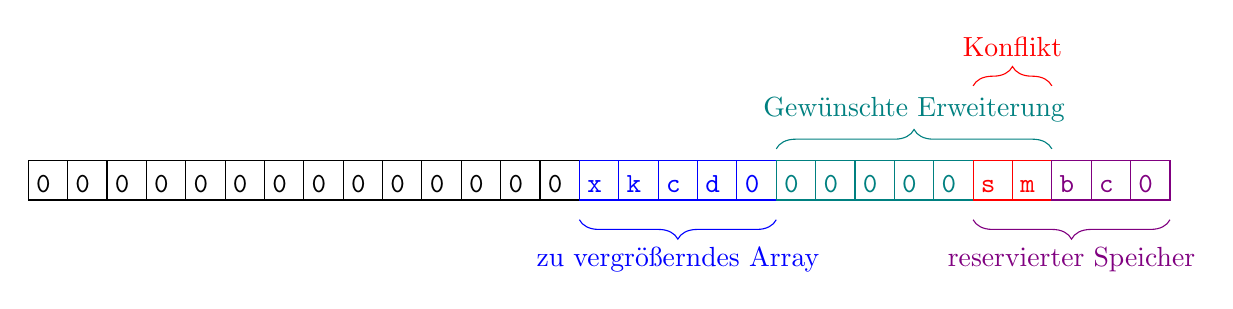
\begin{tikzpicture}
  [ 
    cell/.style={
       text width =3mm,
       text height=3mm, 
       draw=black, 
       inner sep=1mm
    },
    ld/.style={
       draw=blue,
       shorten >=2pt,
       ->
    }
  ]
  \node (c00) at ( 0.0,1) [cell]         {\ttfamily 0};
  \node (c01) at ( 0.5,1) [cell]         {\ttfamily 0};
  \node (c02) at ( 1.0,1) [cell]         {\ttfamily 0};
  \node (c03) at ( 1.5,1) [cell]         {\ttfamily 0};
  \node (c04) at ( 2.0,1) [cell]         {\ttfamily 0};
  \node (c05) at ( 2.5,1) [cell]         {\ttfamily 0};
  \node (c06) at ( 3.0,1) [cell]         {\ttfamily 0};
  \node (c07) at ( 3.5,1) [cell]         {\ttfamily 0};
  \node (c08) at ( 4.0,1) [cell]         {\ttfamily 0};
  \node (c09) at ( 4.5,1) [cell]         {\ttfamily 0};
  \node (c10) at ( 5.0,1) [cell]         {\ttfamily 0};
  \node (c11) at ( 5.5,1) [cell]         {\ttfamily 0};
  \node (c12) at ( 6.0,1) [cell]         {\ttfamily 0};
  \node (c13) at ( 6.5,1) [cell]         {\ttfamily 0};
  \node (c14) at ( 7.0,1) [cell, blue]   {\ttfamily x};
  \node (c15) at ( 7.5,1) [cell, blue]   {\ttfamily k};
  \node (c16) at ( 8.0,1) [cell, blue]   {\ttfamily c};
  \node (c17) at ( 8.5,1) [cell, blue]   {\ttfamily d};
  \node (c18) at ( 9.0,1) [cell, blue]   {\ttfamily 0};
  \node (c19) at ( 9.5,1) [cell, teal]   {\ttfamily 0};
  \node (c20) at (10.0,1) [cell, teal]   {\ttfamily 0};
  \node (c21) at (10.5,1) [cell, teal]   {\ttfamily 0};
  \node (c22) at (11.0,1) [cell, teal]   {\ttfamily 0};
  \node (c23) at (11.5,1) [cell, teal]   {\ttfamily 0};
  \node (c24) at (12.0,1) [cell, red]    {\ttfamily s};
  \node (c25) at (12.5,1) [cell, red]    {\ttfamily m};
  \node (c26) at (13.0,1) [cell, violet] {\ttfamily b};
  \node (c27) at (13.5,1) [cell, violet] {\ttfamily c};
  \node (c28) at (14.0,1) [cell, violet] {\ttfamily 0};
  
  \draw [decorate, decoration={brace,amplitude=7pt, mirror}, xshift=-0pt, yshift=0pt, blue]
  		( 6.75, 0.5) -- ( 9.25, 0.5) node [blue, midway, yshift=-0.5cm] 
		(braceArrayPreResize) {zu vergrößerndes Array};

  \draw [decorate, decoration={brace,amplitude=7pt, mirror}, xshift=-0pt, yshift=0pt, violet]
  		(11.75, 0.5) -- (14.25, 0.5) node [violet, midway, yshift=-0.5cm] 
		(braceArrayPreResize) {reservierter Speicher};

  \draw [decorate, decoration={brace,amplitude=7pt}, xshift=-0pt, yshift=0pt, teal]
  		( 9.25, 1.4) -- (12.75, 1.4) node [teal, midway, yshift=+0.5cm] 
		(braceArrayPreResize) {Gewünschte Erweiterung};

  \draw [decorate, decoration={brace,amplitude=7pt}, xshift=-0pt, yshift=0pt, red]
  		(11.75, 2.2) -- (12.75, 2.2) node [red, midway, yshift=+0.5cm] 
		(braceArrayPreResize) {Konflikt};
\end{tikzpicture}

Stattdessen wird also das Array als Ganzes an eine neue Stelle kopiert:

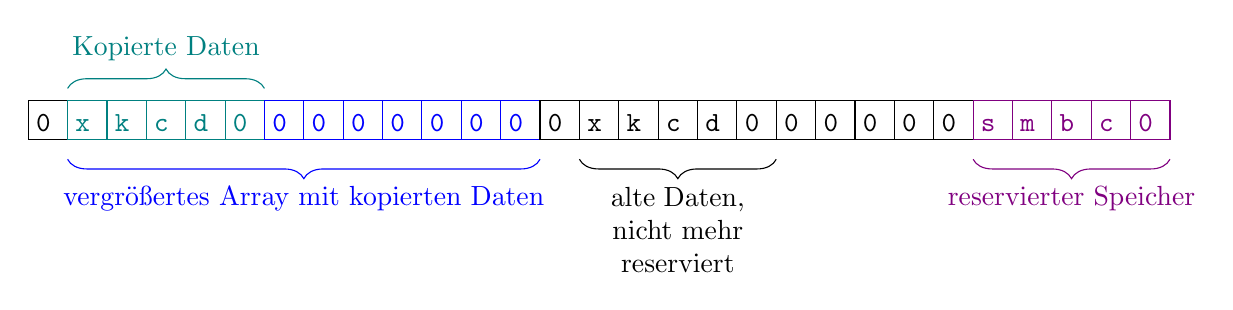
\begin{tikzpicture}
  [ 
    cell/.style={
       text width =3mm,
       text height=3mm, 
       draw=black, 
       inner sep=1mm
    },
    ld/.style={
       draw=blue,
       shorten >=2pt,
       ->
    }
  ]
  \node (c00) at ( 0.0,1) [cell]         {\ttfamily 0};
  \node (c01) at ( 0.5,1) [cell, teal]   {\ttfamily x};
  \node (c02) at ( 1.0,1) [cell, teal]   {\ttfamily k};
  \node (c03) at ( 1.5,1) [cell, teal]   {\ttfamily c};
  \node (c04) at ( 2.0,1) [cell, teal]   {\ttfamily d};
  \node (c05) at ( 2.5,1) [cell, teal]   {\ttfamily 0};
  \node (c06) at ( 3.0,1) [cell, blue]   {\ttfamily 0};
  \node (c07) at ( 3.5,1) [cell, blue]   {\ttfamily 0};
  \node (c08) at ( 4.0,1) [cell, blue]   {\ttfamily 0};
  \node (c09) at ( 4.5,1) [cell, blue]   {\ttfamily 0};
  \node (c10) at ( 5.0,1) [cell, blue]   {\ttfamily 0};
  \node (c11) at ( 5.5,1) [cell, blue]   {\ttfamily 0};
  \node (c12) at ( 6.0,1) [cell, blue]   {\ttfamily 0};
  \node (c13) at ( 6.5,1) [cell]         {\ttfamily 0};
  \node (c14) at ( 7.0,1) [cell]         {\ttfamily x};
  \node (c15) at ( 7.5,1) [cell]         {\ttfamily k};
  \node (c16) at ( 8.0,1) [cell]         {\ttfamily c};
  \node (c17) at ( 8.5,1) [cell]         {\ttfamily d};
  \node (c18) at ( 9.0,1) [cell]         {\ttfamily 0};
  \node (c19) at ( 9.5,1) [cell]         {\ttfamily 0};
  \node (c20) at (10.0,1) [cell]         {\ttfamily 0};
  \node (c21) at (10.5,1) [cell]         {\ttfamily 0};
  \node (c22) at (11.0,1) [cell]         {\ttfamily 0};
  \node (c23) at (11.5,1) [cell]         {\ttfamily 0};
  \node (c24) at (12.0,1) [cell, violet] {\ttfamily s};
  \node (c25) at (12.5,1) [cell, violet] {\ttfamily m};
  \node (c26) at (13.0,1) [cell, violet] {\ttfamily b};
  \node (c27) at (13.5,1) [cell, violet] {\ttfamily c};
  \node (c28) at (14.0,1) [cell, violet] {\ttfamily 0};
  
  \draw [decorate, decoration={brace,amplitude=7pt, mirror}, xshift=-0pt, yshift=0pt, blue]
  		( 0.25, 0.5) -- ( 6.25, 0.5) node [blue, midway, yshift=-0.5cm] 
		(braceArrayPreResize) {vergrößertes Array mit kopierten Daten};

  \draw [decorate, decoration={brace,amplitude=7pt, mirror}, xshift=-0pt, yshift=0pt, violet]
  		(11.75, 0.5) -- (14.25, 0.5) node [violet, midway, yshift=-0.5cm] 
		(braceArrayPreResize) {reservierter Speicher};

  \draw [decorate, decoration={brace,amplitude=7pt}, xshift=-0pt, yshift=0pt, teal]
  		( 0.25, 1.4) -- ( 2.75, 1.4) node [teal, midway, yshift=+0.5cm] 
		(braceArrayPreResize) {Kopierte Daten};
  
  \draw [decorate, decoration={brace,amplitude=7pt, mirror}, xshift=-0pt, yshift=0pt, black]
  		( 6.75, 0.5) -- ( 9.25, 0.5) node [black, midway, yshift=-0.9cm] 
		(braceArrayPreResize) {\parbox{1.7cm}{\centering alte Daten, nicht mehr reserviert}};
\end{tikzpicture}

Da die Daten des Arrays vor dem Vergrößern kopiert (im Gegensatz zu verschoben) werden, bleiben diese Werte in den Speicherzellen. Die Zellen sind aber nicht mehr reserviert. Eine folgende Anfrage, Speicher zu allozieren (\eg mit \texttt{malloc}) kann also genau diese Zellen auswählen und für neue Zwecke benutzen.
\end{tcolorbox}
\begin{tcolorbox}
Verkürzt man ein Array, so wird ebenso lediglich die Reservierung aufgehoben:

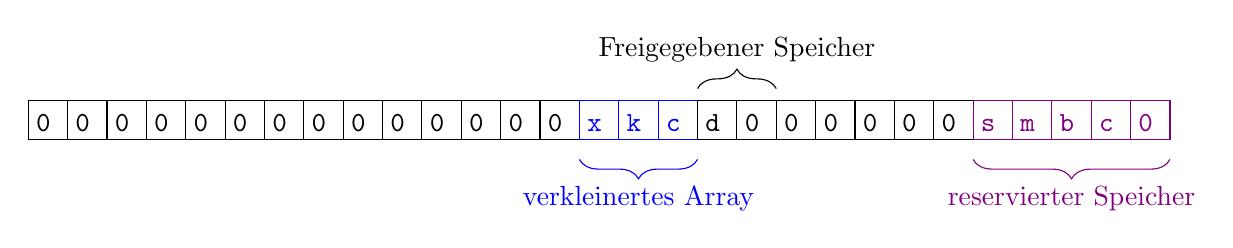
\begin{tikzpicture}
  [ 
    cell/.style={
       text width =3mm,
       text height=3mm, 
       draw=black, 
       inner sep=1mm
    },
    ld/.style={
       draw=blue,
       shorten >=2pt,
       ->
    }
  ]
  \node (c00) at ( 0.0,1) [cell]         {\ttfamily 0};
  \node (c01) at ( 0.5,1) [cell]         {\ttfamily 0};
  \node (c02) at ( 1.0,1) [cell]         {\ttfamily 0};
  \node (c03) at ( 1.5,1) [cell]         {\ttfamily 0};
  \node (c04) at ( 2.0,1) [cell]         {\ttfamily 0};
  \node (c05) at ( 2.5,1) [cell]         {\ttfamily 0};
  \node (c06) at ( 3.0,1) [cell]         {\ttfamily 0};
  \node (c07) at ( 3.5,1) [cell]         {\ttfamily 0};
  \node (c08) at ( 4.0,1) [cell]         {\ttfamily 0};
  \node (c09) at ( 4.5,1) [cell]         {\ttfamily 0};
  \node (c10) at ( 5.0,1) [cell]         {\ttfamily 0};
  \node (c11) at ( 5.5,1) [cell]         {\ttfamily 0};
  \node (c12) at ( 6.0,1) [cell]         {\ttfamily 0};
  \node (c13) at ( 6.5,1) [cell]         {\ttfamily 0};
  \node (c14) at ( 7.0,1) [cell, blue]   {\ttfamily x};
  \node (c15) at ( 7.5,1) [cell, blue]   {\ttfamily k};
  \node (c16) at ( 8.0,1) [cell, blue]   {\ttfamily c};
  \node (c17) at ( 8.5,1) [cell]         {\ttfamily d};
  \node (c18) at ( 9.0,1) [cell]         {\ttfamily 0};
  \node (c19) at ( 9.5,1) [cell]         {\ttfamily 0};
  \node (c20) at (10.0,1) [cell]         {\ttfamily 0};
  \node (c21) at (10.5,1) [cell]         {\ttfamily 0};
  \node (c22) at (11.0,1) [cell]         {\ttfamily 0};
  \node (c23) at (11.5,1) [cell]         {\ttfamily 0};
  \node (c24) at (12.0,1) [cell, violet] {\ttfamily s};
  \node (c25) at (12.5,1) [cell, violet] {\ttfamily m};
  \node (c26) at (13.0,1) [cell, violet] {\ttfamily b};
  \node (c27) at (13.5,1) [cell, violet] {\ttfamily c};
  \node (c28) at (14.0,1) [cell, violet] {\ttfamily 0};
  
  \draw [decorate, decoration={brace,amplitude=7pt, mirror}, xshift=-0pt, yshift=0pt, blue]
  		( 6.75, 0.5) -- ( 8.25, 0.5) node [blue, midway, yshift=-0.5cm] 
		(braceArrayPreResize) {verkleinertes Array};

  \draw [decorate, decoration={brace,amplitude=7pt, mirror}, xshift=-0pt, yshift=0pt, violet]
  		(11.75, 0.5) -- (14.25, 0.5) node [violet, midway, yshift=-0.5cm] 
		(braceArrayPreResize) {reservierter Speicher};

  \draw [decorate, decoration={brace,amplitude=7pt}, xshift=-0pt, yshift=0pt, black]
  		( 8.25, 1.4) -- ( 9.25, 1.4) node [black, midway, yshift=+0.5cm] 
		(braceArrayPreResize) {Freigegebener Speicher};
\end{tikzpicture}
\end{tcolorbox}

In der Syntax orientiert sich \texttt{realloc} am Befehl \texttt{malloc}:

\begin{codebox}[Syntax: \texttt{realloc}]
\begin{minted}{c}
pointer = realloc(pointer, AnzahlBytesNeu);
\end{minted}
\end{codebox}

Dabei ist \texttt{pointer} die Adresse des Arrays, dessen Größe geändert werden soll und \texttt{AnzahlBytesNeu} die gewünschte Größe des neuen Arrays.

Wie wir gesehen haben kann sich die Adresse des Arrays (also sein Startpunkt im Speicher) bei Größenänderung verschieben. Daher müssen wir auch hier das Ergebnis speichern; wir aktualisieren also den Wert der Variablen \texttt{pointer}. Natürlich kann es auch geschehen, dass die Größenänderung fehlschlägt (etwa, wenn ein zu großer Speicherbereich angefragt wird). In diesem Fall ist der Rückgabewert von \texttt{realloc} gleich \texttt{0}. Es gehört zum guten Stil, auf solche Fehler mit \mintinline{c}{if} zu reagieren.

Betrachten wir folgendes Beispiel aus der \href{https://en.cppreference.com/w/c/memory/realloc}{CPP-Referenz}:

\begin{codebox}[Beispiel: \texttt{realloc}]
\begin{minted}[linenos]{c}
#include <stdio.h>
#include <stdlib.h>
 
int main(void) {
    int *pa = malloc(10 * sizeof(*pa)); // allocate an array of 10 int
    if (pa) {
        printf("%ld bytes allocated. Storing ints: ", 10 * sizeof(int));
        for(int n = 0; n < 10; ++n) {printf("%d ", pa[n] = n);}
    }
    
    // reallocate array to a larger size
    int *pb = realloc(pa, 1000000 * sizeof(*pb)); 
    if (pb) {
        printf("\n%ld bytes allocated, first 10 ints are: ", 
               1000000 * sizeof(int)
        );
        for(int n = 0; n < 10; ++n) {printf("%d ", pb[n]);} // show the array
        free(pb);
    } else { // if realloc failed, the original pointer needs to be freed
        free(pa);
    }
}
\end{minted}
{\normalfont(Mit leichten Abwandlungen übernommen von \url{https://en.cppreference.com/w/c/memory/realloc})}
\end{codebox}

\begin{cmdbox}[Ausführungsbeispiel: \texttt{realloc}]
40 bytes allocated. Storing ints: 0 1 2 3 4 5 6 7 8 9 \\
4000000 bytes allocated, first 10 ints are: 0 1 2 3 4 5 6 7 8 9 0
\end{cmdbox}

In Zeile 5 wird versucht, mit \texttt{malloc} Speicher für ein Array zu reservieren, das 10 \mintinline{c}{int}-Werte fassen kann. Beachten Sie hier auch die Verwendung des \mintinline{c}{sizeof}-Operators: Abgefragt wird hier die Speichergröße von \texttt{*pa}. Die Variable \texttt{pa} ist ein Pointer auf \mintinline{c}{int}; damit ist die dereferenzierte Variable \texttt{*pa} selbst ein Ausdruck vom Typ \mintinline{c}{int}.

\emph{Nur wenn diese Allozierung erfolgreich war}, wird das Array mit Werten befüllt und diese Werte zugleich auch auf dem Bildschirm ausgebeben. Beachten Sie hierbei die \texttt{printf}-Anweisung in Zeile 8: Ausgegeben wird der Ausdruck \texttt{pa[n] = n}. Dieser Ausdruck ist zunächst eine \emph{Wertzuweisung} -- in \texttt{pa[n]} wird also der Wert \texttt{n} gespeichert. Zugleich ist das \enquote{Ergebnis} dieser Wertzuweisung der zugewiesene Wert selbst -- \texttt{printf} gibt also den Wert von \texttt{n} aus.

In Zeile 12 versuchen wir nun, das Array so zu vergrößern, dass es \mbox{1\;000\;000} \mintinline{c}{int}-Werte halten kann. Wenn dies gelingt, wird die Variable \texttt{pb} einen von null verschiedenen Wert haben; der Pointer \texttt{pa} dagegen ist \emph{möglicherweise nicht mehr gültig}!

Bei Erfolg dieser Vergrößerung können wir nun über \texttt{pb} auf die Werte des Arrays zugreifen, und finden die Elemente, die wir zuvor über \texttt{pa} gespeichert hatten. Obwohl im Programm zwei verschiedene Pointer-Variablen benutzt werden, existiert nur ein einzeiges Array.

Wie üblich müssen \emph{dynamische Arrays} mit \texttt{free} freigegeben werden. War die Vergrößerung mit \texttt{realloc} erfolgreich, so muss dies über den Pointer \texttt{pb} geschehen, da \texttt{pa} möglicherweise \enquote{ins Leere} zeigt. Konnte dagegen das Array nicht so weit vergrößert werden, so existiert weiterhin das Array mit der Adresse \texttt{pa}. Daher schreiben wir für diesen Fall in Zeile 20 \texttt{free(pa)}.

\subsection{Heap und Stack} \label{sec:HeapStack}
In Abschnitt \ref{sec:Arrays} haben wir \emph{automatische Arrays} kennen gelernt. Später in Abschnitt \ref{sec:dynArrays} haben wir \emph{dynamische Arrays} eingeführt. Während der Zugriff auf die Array-Elemente für beide Arten gleich ist, bestehen doch Unterschiede. \emph{Automatische} Arrays sind in ihrer Größe fest und können nach dem Anlegen nicht mehr verändert werden. Dafür müssen wir uns nicht um die Freigabe des Speichers nach Benutzung kümmern. Für \emph{dynamische} Arrays gilt in dieser Hinsicht das Gegenteil.

Um grob zu verstehen, warum das so ist, müssen Sie wissen, dass der Arbeitsspeicher in mehrere Segmente geteilt wird. 

Ein erstes Segment ist der Code-Bereich. Hier liegt der Maschinencode, also die Folge von Bytes, die den Prozessor Anweisen, unsere Anweisungen auszuführen. 

Hieran schließt sich der \emph{Heap} (englisch: Haufen) an. Es ist ein Bereich, auf den mehr oder minder \enquote{wahllos} zugegriffen werden kann: beliebige Schnitte des Heaps können reserviert und wieder freigegeben werden, ohne eine bestimmte Struktur oder Reihenfolge einhalten zu müssen. Auf dem Heap \enquote{leben} die dynamischen Arrays. Da im allgemeinen nicht vorhergesehen werden kann, wie sich ein dynamisches Array verhält, macht es keinen Sinn, diese geordnet im Speicher unterbringen zu wollen. Zu jeder Zeit könnte ein \texttt{realloc} eine geordnete Struktur aufbrechen. Die reservierten Speicherbereiche liegen also wirklich wie ein ungeordneter Haufen vor.

Der \emph{Stack} dagegen ist eine geordnete Speicherstruktur: Hier liegen alle Werte dicht an dicht, wie Schichten eines geordneten Stapels. Dies ist nur möglich, wenn die einzelnen Schichten nicht ihre Größe ändern (und damit Lücken hinterlassen oder andere Schichten zum nachrücken zwingen). Neue Elemente können nur \enquote{oben auf den Stack gelegt} werden. Zum Freigeben des Speichers muss in umgekehrter Reihenfolge vorgegangen werden, der Stack wird \enquote{von oben nach unten} freigegeben. Auf dem Stack \enquote{leben} die automatischen Variablen, \ie Arrays wie in Abschnitt \ref{sec:Arrays} gezeigt, aber auch die \enquote{normalen Variablen}, die nur einen einzelnen Wert halten können.

\begin{tcolorbox}[title=Visualisierung: Heap und Stack]
\begin{tikzpicture}
\footnotesize
\node (code) 
	[text height=3mm, text depth=3mm, text width=.2\linewidth, fill=red!50!white]
	{Code};
\node (heap) 
	[text height=3mm, text depth=3mm, text width=.3\linewidth, fill=green!50!white, right=0pt of code] 
	{Heap};
\node (stack) 
	[text height=3mm, text depth=3mm, text width=.2\linewidth, fill=blue!50!white,  right=0pt of heap] 
	{Stack};
	
\node (tcode) 
	[below=2mm of code, text width=.18\linewidth, font=\rightskip0pt plus 1fil]
	{Programmcode -- kompilierte Datei};
\node (theap) 
	[below=2mm of heap, text width=.23\linewidth, font=\rightskip0pt plus 1fil]
	{Dynamische Speicherverwaltung};
\node (tstack) 
	[below=2mm of stack,text width=.18\linewidth, font=\rightskip0pt plus 1fil]
	{Automatische Variablen};
\end{tikzpicture}
%\\
\hspace{10pt}
\includegraphics[width=.2\linewidth]{./gfx/Stack}
\end{tcolorbox}

Da der Stack eine so regelmäßige Gestalt hat, kann die Verwaltung automatisiert vom Betriebssystem übernommen werden. Wir müssen lediglich die Variablen deklarieren, jedoch nicht explizit Speicherplatz allozieren oder freigeben.

\begin{warnbox}[Keine dynamischen Operationen an automatischen Variablen]
Operationen der dynamischen Speicherverwaltung (insbesondere die Befehle \texttt{realloc} und \texttt{free}) sind auf dem Stack nicht erlaubt. Daher darf \emph{niemals} die Größe eines automatischen Arrays mit \texttt{realloc} geändert werden und auch \emph{niemals} sein Speicher mit \texttt{free} freigegeben werden. Der Versuch, dies zu tun führt sofort zum Programmabsturz.
\end{warnbox}


\subsection{C++} \label{sec:ArrayCPP}
\begin{plusbox}
Wie üblich stehen auch in C++ alle soeben gezeigten Mittel zur Verfügung. Automatische Arrays werden ebenso angelegt wie in C. Für \emph{dynamische Arrays} dagegen sollten nicht mehr \texttt{malloc}, \texttt{calloc} und \texttt{free} verwendet werden, sondern die Operatoren \mintinline{c++}{new} und \mintinline{c++}{delete}.

Die Syntax lautet:

\begin{codebox}[Syntax: \texttt{new} und \texttt{delete}]
\begin{minted}{c++}
pointer = new datatype [AnzahlFelder];
...
delete pointer;
\end{minted}
\end{codebox}

Auf die Unterschiede kann an dieser Stelle leider nicht im Detail eingegangen werden.

Stattdessen sei hier vermerkt, dass die C++ Standard Library eine Vielzahl von Mitteln zur Verfügung stellt, die den \emph{direkten Umgang} mit Pointern unnötig machen. Diese Mittel werden in einem eigenen Kurs vorgestellt und sind den C-Arrays \idR klar vorzuziehen.
\end{plusbox}

\subsection{mehrdimensionale dynamische Arrays}
In Abschnitt \ref{sec:MultiDimArray} haben wir bereits gesehen, wie mehrdimensionale Objekte wie Tabellen im Speicher organisiert werden können. An dieser Stelle möchte ich zwei Techniken besprechen, die solche Objekte auch mit dynamischen Arrays verfügbar machen.

\subsubsection{Geplättete Listen}
Der sicher einfachste Weg ist es, eine Tabelle (oder sein höherdimensionales Objekt) zu \enquote{plätten}, also die einzelnen Listen, aus denen es besteht, hintereinander im Speicher anzuordnen. In diesem Fall muss zwar für jeden Zugriff aus den \enquote{Koordinaten} (also \eg Spalten- und Zeilennummern der Tabelle) ein Index berechnet werden. Der sonstige \emph{Overhead} (Verwaltungsaufwand) hält sich jedoch in Grenzen.

Folgendes Beispiel erzeugt eine Tabelle, deren Maße vom User bestimmt werden, und befüllt die Zellen mit ihren Indizes. Anschließend wird die Tabelle auf dem Bildschirm ausgegeben:

\begin{codebox}[Beispiel: Tabelle mit dynamischem Array]
\begin{minted}[linenos]{c}
#include <stdio.h>
#include <stdlib.h>
 
int main(void) {
  int width = -1, height = -1, i, r, c;
  
  // Usereingaben
  printf("Bitte geben Sie die Breite der Tabelle ein:\n");
  scanf("%d", &width);
  
  printf("Bitte geben Sie die Höhe der Tabelle ein:\n");
  scanf("%d", &height);
  
  if ((height <= 0) || (width <= 0)) {
    printf("Ungültige Eingabe -- Programm wird beendet.\n");
    exit(-1);
  }
  
  // Speicher für Tabelle allozieren
  int * table = malloc(width * height * sizeof(*table));
  if (!table) {
    printf("Allozierung fehlgeschlagen -- Programm wird beendet.\n");
    exit(-1);
  }
  
  // Tabelleninhalt schreiben
  for (i = 0; i < width * height; i++) {
    table[i] = i;
  }
  
  // Tabelle auf dem Bildschirm ausgeben
  for   (r = 0; r < height; r++) {
    for (c = 0; c < width;  c++) {
      printf("%3d\t", table[r * width + c]);
    }
    printf("\n");
  }
  
  // Speicher freigeben
  free(table);
}
\end{minted}
\end{codebox}

\begin{cmdbox}[Ausgabebeispiel: Tabelle mit dynamischem Array]
\begin{minted}{text}
Bitte geben Sie die Breite der Tabelle ein:
5
Bitte geben Sie die Höhe der Tabelle ein:
3
  0       1       2       3       4
  5       6       7       8       9
 10      11      12      13      14
\end{minted}
\end{cmdbox}

Das Array \texttt{table}, in dem wir unsere Tabelle geplättet ablegen, kann mit \texttt{realloc} vergrößert und verkleinert werden. Soll die Struktur der Tabelle erhalten bleiben, können wir auf dieses Mittel allerdings nicht zurückgreifen.

Ausgehend vom obigen Code (\emph{Tabelle mit dynamischem Array}) ändern wir das Ende des Codes ab und versuchen, ab Zeile 39 die Tabelle um eine Spalte zu verbreitern:

\begin{warnbox}[Beispiel: Tabelle vergrößern mit dynamischem Array -- (fehlerhafter Code),leftupper=7mm]
\begin{minted}[linenos, firstnumber=39]{c}
  // Tabelle verbreitern
  width++;
  int * newTable = realloc(table, width * height * sizeof(*table));
  if (!newTable) {
    printf("Allozierung fehlgeschlagen -- Programm wird beendet.\n");
    free(table);
    exit(-1);
  } else {
    table = newTable;
  }
  
  // Tabelle auf dem Bildschirm ausgeben
  printf("\nVerbreiterte Tabelle:\n");
  for   (r = 0; r < height; r++) {
    for (c = 0; c < width;  c++) {
      printf("%3d\t", table[r * width + c]);
    }
    printf("\n");
  }
  
  // Speicher freigeben
  free(table);
}
\end{minted}
\end{warnbox}

Die Ausgabe lautet:

\begin{cmdbox}[Ausgabebeispiel: Tabelle vergrößern mit dynamischem Array -- (fehlerhafter Code)]
\begin{minted}{text}
Bitte geben Sie die Breite der Tabelle ein:
5
Bitte geben Sie die Höhe der Tabelle ein:
3
  0       1       2       3       4
  5       6       7       8       9
 10      11      12      13      14

Verbreiterte Tabelle:
  0       1       2       3       4       5
  6       7       8       9      10      11
 12      13      14       0       0       0

\end{minted}
\end{cmdbox}

Um dieses Verhalten zu verstehen, müssen wir uns das Speicherbild ansehen:

\begin{tcolorbox}[title=Visualisierung: Abbild der Tabelle im Speicher]
Bis Zeile 39 des Codes liegen die Tabellen-Zeilen dicht aneinander:

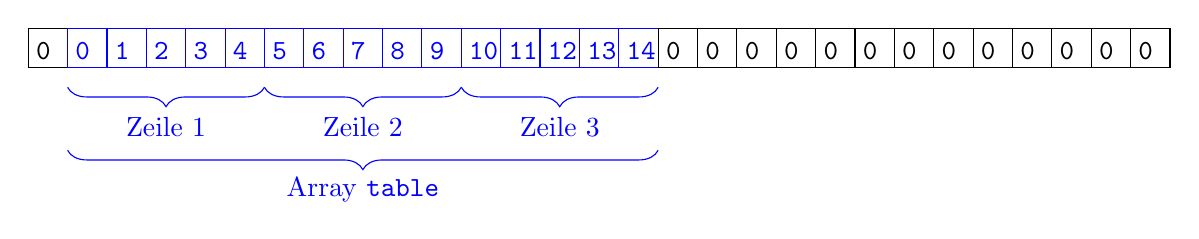
\begin{tikzpicture}
  [ 
    cell/.style={
       text width =3mm,
       text height=3mm, 
       draw=black, 
       inner sep=1mm
    },
    ld/.style={
       draw=blue,
       shorten >=2pt,
       ->
    }
  ]
  \node (c00) at ( 0.0,1) [cell]         {\ttfamily  0};
  \node (c01) at ( 0.5,1) [cell, blue]   {\ttfamily  0};
  \node (c02) at ( 1.0,1) [cell, blue]   {\ttfamily  1};
  \node (c03) at ( 1.5,1) [cell, blue]   {\ttfamily  2};
  \node (c04) at ( 2.0,1) [cell, blue]   {\ttfamily  3};
  \node (c05) at ( 2.5,1) [cell, blue]   {\ttfamily  4};
  \node (c06) at ( 3.0,1) [cell, blue]   {\ttfamily  5};
  \node (c07) at ( 3.5,1) [cell, blue]   {\ttfamily  6};
  \node (c08) at ( 4.0,1) [cell, blue]   {\ttfamily  7};
  \node (c09) at ( 4.5,1) [cell, blue]   {\ttfamily  8};
  \node (c10) at ( 5.0,1) [cell, blue]   {\ttfamily  9};
  \node (c11) at ( 5.5,1) [cell, blue]   {\ttfamily 10};
  \node (c12) at ( 6.0,1) [cell, blue]   {\ttfamily 11};
  \node (c13) at ( 6.5,1) [cell, blue]   {\ttfamily 12};
  \node (c14) at ( 7.0,1) [cell, blue]   {\ttfamily 13};
  \node (c15) at ( 7.5,1) [cell, blue]   {\ttfamily 14};
  \node (c16) at ( 8.0,1) [cell]         {\ttfamily  0};
  \node (c17) at ( 8.5,1) [cell]         {\ttfamily  0};
  \node (c18) at ( 9.0,1) [cell]         {\ttfamily  0};
  \node (c19) at ( 9.5,1) [cell]         {\ttfamily  0};
  \node (c20) at (10.0,1) [cell]         {\ttfamily  0};
  \node (c21) at (10.5,1) [cell]         {\ttfamily  0};
  \node (c22) at (11.0,1) [cell]         {\ttfamily  0};
  \node (c23) at (11.5,1) [cell]         {\ttfamily  0};
  \node (c24) at (12.0,1) [cell]         {\ttfamily  0};
  \node (c25) at (12.5,1) [cell]         {\ttfamily  0};
  \node (c26) at (13.0,1) [cell]         {\ttfamily  0};
  \node (c27) at (13.5,1) [cell]         {\ttfamily  0};
  \node (c28) at (14.0,1) [cell]         {\ttfamily  0};
  
  \draw [decorate, decoration={brace,amplitude=7pt, mirror}, xshift=-0pt, yshift=0pt, blue]
  		( 0.25, -0.3) -- ( 7.75, -0.3) node [blue, midway, yshift=-0.5cm] 
		(braceArrayPreResize) {Array \texttt{table}};

  \draw [decorate, decoration={brace,amplitude=7pt, mirror}, xshift=-0pt, yshift=0pt, blue]
  		( 0.25, 0.5) -- ( 2.75, 0.5) node [blue, midway, yshift=-0.5cm] 
		(braceArrayPreResize) {Zeile 1};
  \draw [decorate, decoration={brace,amplitude=7pt, mirror}, xshift=-0pt, yshift=0pt, blue]
  		( 2.75, 0.5) -- ( 5.25, 0.5) node [blue, midway, yshift=-0.5cm] 
		(braceArrayPreResize) {Zeile 2};
  \draw [decorate, decoration={brace,amplitude=7pt, mirror}, xshift=-0pt, yshift=0pt, blue]
  		( 5.25, 0.5) -- ( 7.75, 0.5) node [blue, midway, yshift=-0.5cm] 
		(braceArrayPreResize) {Zeile 3};
\end{tikzpicture}

Mit \texttt{realloc} erweitern wir unseren Speicher um weitere 3 Elemente, um so Platz für eine zusätzliche Spalte zu haben. Wie in Abschnitt \ref{sec:realloc} gezeigt, wird dieser Platz \emph{am Ende des Arrays} angehängt. Wegen \texttt{width++} in Code-Zeile 48 lesen wir ab jetzt aber Ketten von \emph{6 Speicherstellen} als eine Zeile, und erhalten eine zersetzte Tabelle:

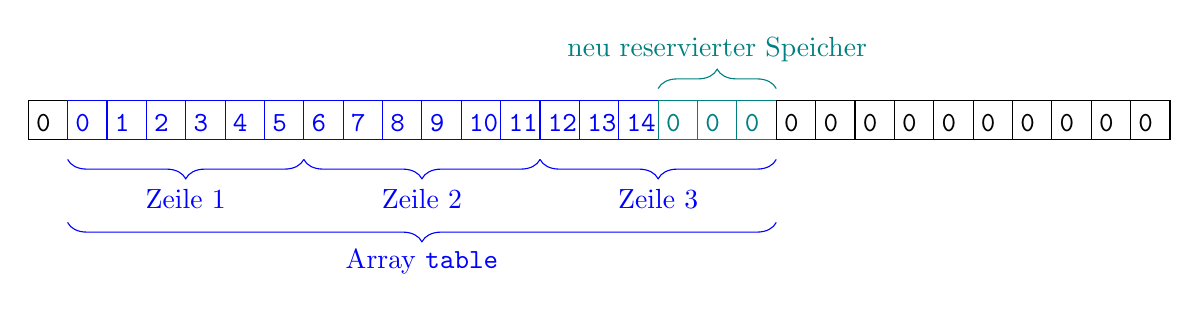
\begin{tikzpicture}
  [ 
    cell/.style={
       text width =3mm,
       text height=3mm, 
       draw=black, 
       inner sep=1mm
    },
    ld/.style={
       draw=blue,
       shorten >=2pt,
       ->
    }
  ]
  \node (c00) at ( 0.0,1) [cell]         {\ttfamily  0};
  \node (c01) at ( 0.5,1) [cell, blue]   {\ttfamily  0};
  \node (c02) at ( 1.0,1) [cell, blue]   {\ttfamily  1};
  \node (c03) at ( 1.5,1) [cell, blue]   {\ttfamily  2};
  \node (c04) at ( 2.0,1) [cell, blue]   {\ttfamily  3};
  \node (c05) at ( 2.5,1) [cell, blue]   {\ttfamily  4};
  \node (c06) at ( 3.0,1) [cell, blue]   {\ttfamily  5};
  \node (c07) at ( 3.5,1) [cell, blue]   {\ttfamily  6};
  \node (c08) at ( 4.0,1) [cell, blue]   {\ttfamily  7};
  \node (c09) at ( 4.5,1) [cell, blue]   {\ttfamily  8};
  \node (c10) at ( 5.0,1) [cell, blue]   {\ttfamily  9};
  \node (c11) at ( 5.5,1) [cell, blue]   {\ttfamily 10};
  \node (c12) at ( 6.0,1) [cell, blue]   {\ttfamily 11};
  \node (c13) at ( 6.5,1) [cell, blue]   {\ttfamily 12};
  \node (c14) at ( 7.0,1) [cell, blue]   {\ttfamily 13};
  \node (c15) at ( 7.5,1) [cell, blue]   {\ttfamily 14};
  \node (c16) at ( 8.0,1) [cell, teal]   {\ttfamily  0};
  \node (c17) at ( 8.5,1) [cell, teal]   {\ttfamily  0};
  \node (c18) at ( 9.0,1) [cell, teal]   {\ttfamily  0};
  \node (c19) at ( 9.5,1) [cell]         {\ttfamily  0};
  \node (c20) at (10.0,1) [cell]         {\ttfamily  0};
  \node (c21) at (10.5,1) [cell]         {\ttfamily  0};
  \node (c22) at (11.0,1) [cell]         {\ttfamily  0};
  \node (c23) at (11.5,1) [cell]         {\ttfamily  0};
  \node (c24) at (12.0,1) [cell]         {\ttfamily  0};
  \node (c25) at (12.5,1) [cell]         {\ttfamily  0};
  \node (c26) at (13.0,1) [cell]         {\ttfamily  0};
  \node (c27) at (13.5,1) [cell]         {\ttfamily  0};
  \node (c28) at (14.0,1) [cell]         {\ttfamily  0};
  
  \draw [decorate, decoration={brace,amplitude=7pt, mirror}, xshift=-0pt, yshift=0pt, blue]
  		( 0.25, -0.3) -- ( 9.25, -0.3) node [blue, midway, yshift=-0.5cm] 
		(braceArrayPreResize) {Array \texttt{table}};

  \draw [decorate, decoration={brace,amplitude=7pt, mirror}, xshift=-0pt, yshift=0pt, blue]
  		( 0.25, 0.5) -- ( 3.25, 0.5) node [blue, midway, yshift=-0.5cm] 
		(braceArrayPreResize) {Zeile 1};
  \draw [decorate, decoration={brace,amplitude=7pt, mirror}, xshift=-0pt, yshift=0pt, blue]
  		( 3.25, 0.5) -- ( 6.25, 0.5) node [blue, midway, yshift=-0.5cm] 
		(braceArrayPreResize) {Zeile 2};
  \draw [decorate, decoration={brace,amplitude=7pt, mirror}, xshift=-0pt, yshift=0pt, blue]
  		( 6.25, 0.5) -- ( 9.25, 0.5) node [blue, midway, yshift=-0.5cm] 
		(braceArrayPreResize) {Zeile 3};

  \draw [decorate, decoration={brace,amplitude=7pt}, xshift=-0pt, yshift=0pt, teal]
  		( 7.75, 1.4) -- ( 9.25, 1.4) node [teal, midway, yshift=+0.5cm] 
		(braceArrayPreResize) {neu reservierter Speicher};
\end{tikzpicture}
\end{tcolorbox}

(Wenn dagegen nur eine Zeile an die Tabelle angehängt werden soll, funktioniert dieses Beispiel mit \texttt{realloc} genau wie erwartet, da neue Zeilen immer \emph{am Ende} der \enquote{geplätteten Liste} angehängt werden.

Um nun auch Spalten anhängen zu können, müssen wir manuell ein neues Array erstellen und alle Tabellen-Einträge an die richtigen Stellen kopieren. Wir gehen wieder vom Beispiel \emph{Tabelle mit dynamischem Array} aus und ergänzen ab Zeile 39:

\begin{codebox}[Beispiel: Tabelle vergrößern mit dynamischem Array -- (korrekter Code)]
\begin{minted}[linenos, firstnumber=39]{c}
  // neue Tabelle anlegen
  int * newTable = calloc((width + 1) * height, sizeof(*table));
  if (!newTable) {
    printf("Allozierung fehlgeschlagen -- Programm wird beendet.\n");
    exit(-1);
  }
  
  // Tabelleninhalt kopieren
  for   (r = 0; r < height; r++) {
    for (c = 0; c < width;  c++) {
      newTable[r * (width + 1) + c] = table[r * width + c];
    }
  }
  
  // Speicher der alten Tabelle freigeben, Variablen aktualisieren
  free(table);
  table = newTable;
  width++;
  
  // Tabelle auf dem Bildschirm ausgeben
  printf("\nVerbreiterte Tabelle:\n");
  for   (r = 0; r < height; r++) {
    for (c = 0; c < width;  c++) {
      printf("%3d\t", table[r * width + c]);
    }
    printf("\n");
  }
  
  // Speicher freigeben
  free(table);
}
\end{minted}
\end{codebox}

\begin{cmdbox}[Ausgabebeispiel: Tabelle vergrößern mit dynamischem Array -- (korrekter Code)]
\begin{minted}{text}
Bitte geben Sie die Breite der Tabelle ein:
5
Bitte geben Sie die Höhe der Tabelle ein:
3
  0       1       2       3       4
  5       6       7       8       9
 10      11      12      13      14

Verbreiterte Tabelle:
  0       1       2       3       4       0
  5       6       7       8       9       0
 10      11      12      13      14       0
\end{minted}
\end{cmdbox}

\subsubsection{Pointer zweiter und tieferer Ebene}
Wir haben bereits festgestellt, dass sich eine Tabelle auch als \emph{Liste von Listen} auffassen lässt. Listen werden mit Pointern verwaltet. Die Sprache C erlaubt auch, \emph{Pointer auf Pointer} anzulegen. Diesem Gedanken folgend wollen wir eine alternative Darstellungsmöglichkeit von Tabellen diskutieren:

\begin{codebox}[Beispiel: Tabelle Pointer zweiter Ebene]
\begin{minted}[linenos]{c}
#include <stdio.h>
#include <stdlib.h>
 
int main(void) {
  int width  = -1, height = -1, r, c;
  
  // Usereingaben
  printf("Bitte geben Sie die Breite der Tabelle ein:\n"); scanf("%d", &width);
  printf("Bitte geben Sie die Höhe der Tabelle ein:\n");   scanf("%d", &height);
  
  if ((height <= 0) || (width <= 0)) {
    printf("Ungültige Eingabe -- Programm wird beendet.\n");
    exit(-1);
  }
  
  // Speicher für Tabelle allozieren
  int ** table = malloc(height * sizeof(*table));         // Liste der Zeilen
  if (!table) {
    printf("Allozierung fehlgeschlagen -- Programm wird beendet.\n");
    exit(-1);
  }
  for (r = 0; r < height; r++) {
    table[r] = malloc(  width * sizeof(*(table[r]))  );   // Zeilen selbst
  }
  
  // Tabelleninhalt schreiben
  for   (r = 0; r < height; r++) {
    for (c = 0; c < width;  c++) {
      table[r][c] = r * width + c;
    }
  }
  
  // Tabelle auf dem Bildschirm ausgeben
  for   (r = 0; r < height; r++) {
    for (c = 0; c < width;  c++) {
      printf("%3d\t", table[r][c]);
    }
    printf("\n");
  }
  
  // Speicher freigeben
  for (r = 0; r < height; r++) {free(table[r]);}
  free(table);
}
\end{minted}
\end{codebox}

Die Ausgabe ist dieselbe wie im vorigen Beispiel (\emph{Tabelle mit dynamischem Array}); \enquote{unter der Haube} sieht es jedoch bedeutend anders aus.

Zeile 17 deklariert einen \mintinline{c}{int **}, also einen \emph{Pointer auf einen \mintinline{c}{int *}}. Diese Variable \texttt{table} verweist also nicht auf den Speicherbereich, in dem die Tabellendaten selbst liegen, sondern auf Punkte im Speicher, die angeben, wo die einzelnen Zeilen der Tabelle zu finden sind.

Für jeden Eintrag in dieser Liste aus Pointern wird nun nochmal ein eigener Speicherbereich alloziert, der die tatsächlichen Tabellenwerte aufnehmen kann (Zeilen 22-24).

Mit diesem aufwändigeren Aufbau der Speicherstruktur können wir nun etwas komfortabler auf die Tabellenelemente zugreifen. In Zeile 29 wird \texttt{table[r][c]} beschrieben, wir geben also direkt den Zeilenindex \texttt{r} und den Spaltenindex \texttt{c} an, ohne einen geplätteten Index berechnen zu müssen. Halten Sie sich vor Augen: \texttt{table} ist ein \mintinline{c}{int **}. Damit liefert der Zugriff \texttt{table[r]} den Wert mit dem Index \texttt{r} aus der \emph{Liste der Listen}, also einen Pointer auf die Zeile \texttt{r}. Auf diese Liste kann nun mit dem Spaltenindex \texttt{c} zugegriffen werden.

Insgesamt haben wir also \texttt{r + 1} Listen, die die Tabelle aufbauen (\texttt{r} Listen für die Inhalte der Zeilen selbst und eine Liste, die angibt, wo im Speicher diese Zeilen zu finden sind). Alle diese Listen müssen natürlich auch wieder freigegeben werden. Hierzu dienen die Zeilen 42 und 43. Wichtig ist, dies in \emph{umgekehrter Reihenfolge des Anlegens} zu tun. Nach einem \texttt{free} \enquote{existiert} ein Array nicht mehr und ein Zugriff darauf darf eigentlich nicht mehr stattfinden. Wenn wir also die Zeilen 42 und 43 vertauschen, würden in der \mintinline{c}{for}-Schleife verbotene Zugriffe auf \texttt{table} stattfinden und möglicherweise den Programmabsturz hervorrufen.

Wollen wir diese Tabelle vergrößern, so gilt es, zwei Fälle zu unterscheiden: Eine Änderung der Zeilen-Zahl oder der Spalten-Zahl. Wenn wir Zeilen hinzufügen, reicht es, lediglich \texttt{table} mit \texttt{realloc} zu vergrößern und mit \texttt{malloc} Platz für diese neuen Zeilen zu allozieren. Für zusätzliche Spalten müssen wir jede Liste \texttt{table[r]} mit \texttt{realloc} vergrößern. Zum Verkleinern solcher Strukturen müssen Sie auch darauf achten, dass wegfallende Zeilen mit \texttt{free(table[r])} freigegeben werden müssen.

\begin{hintbox}[Geplättete Listen bevorzugen]
Wie Sie sehen ist die Verwaltung von Listen mit Pointern zweiter oder höherer Ebene komplexer und bietet mehr Fehlerquellen. Im Allgemeinen sind daher \enquote{geplättete Listen} zu bevorzugen. Relevant kann diese Technik aber dort werden, wo sie keine vollständige, \enquote{rechteckige} Tabelle beschreiben, sondern wo jede Zeile eine andere Länge hat. Für diesen Fall müssen Sie natürlich noch ein zusätzliches Array anlegen, in dem Sie die Längen der Zeilen speichern.
\end{hintbox}

\begin{hintbox}[Reihenfolge der Dimensionen frei wählbar]
In den obigen Beispielen folgte ich der Konvention \enquote{Zeilen zuerst, Spalten später}. Es gibt aber keine zwingenden Gründe hierfür; Sie können die obigen Beispiele leicht so anpassen, dass die Reihenfolge von Zeilen und Spalten vertauscht werden. Die Berechnung der geplätteten Indizes kann gleich bleiben, oder nach der Formel
\[ \mathtt{Index = c * height + r} \]
stattfinden. Dies entspricht einer Spaltenweisen Anordnung im Speicher.

Für welche Anordnung Sie sich auch entscheiden: Behalten Sie eine einmal gewählte Konvention bei, da Sie sonst durch die Verwechslung von Spalten und Zeilen viele Fehler machen werden.

Die hier gezeigten Konventionen orientieren sich an den Gewohnheiten der Mehrheit der ProgrammiererInnen. Für die Arbeit in Teams ist diese Reihenfolge also zu bevorzugen.
\end{hintbox}

\section{C-Strings} \label{sec:string}
Bisher haben wir fast ausschließlich mit Zahlenwerten gearbeitet. Wie wir in Abbildung \ref{fig:ASCII} gesehen haben, sind Buchstaben aber nur \enquote{Interpretationsweisen} von Ganzzahlen. Texte -- Zeichenketten, oder englisch: \emph{Strings} -- lassen sich also mit Ganzzahl-Arrays behandeln. Um diese (häufig auftretende) Aufgabe zu erleichtern bringt die Sprache C einige Mittel für den Umgang mit Strings mit.

\subsection{spezielle Syntax-Elemente}
Für einfache Aufgaben steht uns ein Vorrat aus 256 verschiedenen Zeichen zur Verfügung. Dies ist genau der Wertebereich des Datentyps \mintinline{c}{char} (von englisch: \emph{character}, Buchstabe oder Zeichen). Wir verwenden also \mintinline{c}{char}-Arrays zur Arbeit mit Strings.

Es ist zwar möglich, jeden Buchstaben in der ASCII-Tabelle nachzuschlagen und manuell den zugehörigen Zahlenwert zuzuweisen; jedoch wäre dies reichlich aufwändig und fehleranfällig. Stattdessen können wir auch \texttt{'}einfache Anführungszeichen\texttt{'} benutzen, um \enquote{der Zeichencode für das eingeschlossene Zeichen} auszudrücken.

\begin{codebox}[Beispiel: ASCII-Codes]
\begin{minted}[linenos]{c}
#include <stdio.h>

int main () {
  printf("Der ASCII-Code von 'a' ist %d.\n", 'a');
}
\end{minted}
\end{codebox}

Der Format-String erwartet eine Dezimalzahl (\texttt{\%d}). Um diesen Platzhalter auszufüllen wird der Ausdruck \texttt{'a'} angeboten. Statt also eine (nicht existente) Variable \texttt{a} auszugeben wird der ASCII-Code des Zeichens \texttt{a} gelesen. Entsprechend lautet die Ausgabe:

\begin{cmdbox}[Ausführungsbeispiel: ASCII-Codes]
Der ASCII-Code von 'a' ist 97.
\end{cmdbox}

\begin{hintbox}[Regelmäßigkeit von ASCII-Codes]
Die Anordnung der Zeichen im ASCII-Vorrat ist nicht zufällig. Ein nützliches Ergebnis dieser Anordnung ist, dass sich die Bitmuster von Groß- und Kleinbuchstaben in genau einem Bit unterscheiden. Es ist also möglich, \enquote{auf den ersten Blick} festzustellen, ob eine bestimmte Folge von 1en und 0en einen großen oder einen kleinen Buchstaben beschreibt.

Da Buchstaben nur Interpretationsweisen von Zahlen sind, kann mit diesen auch gerechnet werden wie mit normalen Ganzzahlen. Insbesondere beschreibt der Ausdruck
\begin{center}
\texttt{'a' - 'A'}
\end{center}
damit auch den Abstand zwischen Groß- und Kleinbuchstaben. Der Wert dieses Ausdrucks kann zu jedem Großbuchstaben addiert werden um den entsprechenden Kleinbuchstaben zu finden; umgekehrt wandelt die Subtraktion einen Kleinbuchstaben in einen Großbuchstaben um.
\end{hintbox}

Mit diesem Mittel können wir bereits ein \mintinline{c}{char}-Array anlegen und einen Text darin ablegen:

\begin{codebox}[Beispiel: Wertzuweisung Strings (1)]
\begin{minted}[linenos]{c}
#include <stdio.h>

int main () {
  char string[] = {
    'D', 'u', 'n', 'e', ' ', 'b', 'y', ' ', 
    'F', 'a', 'n', 'k', ' ', 'H', 'e', 'r', 'b', 'e', 'r', 't', 0};
}
\end{minted}
\end{codebox}

Damit legen wir ein automatisches Array namens \texttt{string} an, und speichern darin den Text \texttt{Dune by Frank Herbert}. Die Größe wird durch die Initializer-Syntax automatisch ermittelt und die einfachen Anführungszeichen sorgen dafür, dass die ASCII-Codes richtig zugewiesen werden.

Beachten Sie auch das letzte Zeichen dieses Beispiels: Das Zeichen \texttt{0} (\emph{Null-Char}) wird im Kontext von Zeichenketten benutzt um das Ende eines Strings zu markieren. Der Vorteil hiervon ist, dass man nicht im Vorhinein die Länge eines Strings kennen muss, um sinnvoll mit diesem arbeiten zu können. Bei der Ausgabe auf dem Bildschirm werden beispielsweise so lange Zeichen gedruckt, bis man auf dieses Null-Char stößt. Statt die Zahl \texttt{0} zu schreiben kann auch die \emph{Escape-Sequenz} \texttt{\textbackslash 0} benutzt werden.

Wenn wir nicht nur mit einzelnen Schriftzeichen arbeiten, sondern ganze Zeichen\emph{ketten} bearbeiten,  dann ist auch die oben gezeigte Syntax noch unhandlich. Zu diesem Zweck existiert die Möglichkeit, ganze Zeichenketten in '{}'doppelte Anführungszeichen'{}' zu setzen. Gleichwertig zu obigem Code (\emph{Wertzuweisung Strings (1)}) ist also auch:

\begin{codebox}[Beispiel: Wertzuweisung Strings (2)]
\begin{minted}[linenos]{c}
#include <stdio.h>

int main () {
  char string[] = "Dune by Frank Herbert";
}
\end{minted}
\end{codebox}

Sie sehen: Nicht nur ist dieser Code bedeutend kürzer; sie können auch auf die Nennung des Null-Chars verzichten. Solche Zeichenketten in \texttt{"}doppelten Anführungszeichen\texttt{"} nennen wir \emph{String-Literals}.

Zur Ausgabe von Strings steht uns ein eigenes Formatierungszeichen zur Verfügung. Im Formatstring können wir \texttt{\%s} setzen, um eine Zeichenkette auszugeben. In der Parameterliste wird hier der \emph{Pointer auf das \mintinline{c}{char}-Array} übergeben:

\begin{codebox}[Beispiel: Formattierte Ausgabe von Strings (1)]
\begin{minted}[linenos]{c}
#include <stdio.h>

int main () {
  char string[] = "Dune by Frank Herbert";
  printf("My favourite book is %s.\n", string);
}
\end{minted}
\end{codebox}

\begin{cmdbox}[Ausführungseispiel: Formattierte Ausgabe von Strings (1)]
\begin{minted}{text}
My favourite book is Dune by Frank Herbert.
\end{minted}
\end{cmdbox}

Ähnlich wie auch bei den Zahlentypen kann in einem \texttt{printf}-Formatstring angegeben werden, wie viel Platz für die Ausgabe zur Verfügung gestellt werden soll. Wie schon zuvor erzeugt eine positive Zahl dabei eine rechtsbündige Ausgabe; negative Zahlen halten den Text linksbündig.

\begin{codebox}[Beispiel: Formattierte Ausgabe von Strings (2)]
\begin{minted}[linenos]{c}
#include <stdio.h>

int main () {
  printf("|%s|\n"   , "Dune");
  printf("|%10s|\n" , "Dune");
  printf("|%-10s|\n", "Dune");
}
\end{minted}
\end{codebox}

\begin{cmdbox}[Ausführungseispiel: Formattierte Ausgabe von Strings (2)]
\begin{minted}{text}
|Dune|
|      Dune|
|Dune      |
\end{minted}
\end{cmdbox}

\subsection{User-Eingaben} \label{sec:strInput}
Wir können \texttt{scanf} mit dem Formatstring-Platzhalter \texttt{\%s} benutzen, um den User direkt zur Texteingabe aufzufordern. Dafür muss bereits vor der Eingabe genug Speicherplatz reserviert sein, um die gesamte Usereingabe aufzunehmen. Wie üblich werden Zeilenumbrüche, Tabulatoren und Leerzeichen als Trennzeichen interpretiert:

\begin{codebox}[Beispiel: Strings mit scanf einlesen (1)]
\begin{minted}[linenos]{c}
#include <stdio.h>

int main () {
  char userinput[1024];
  
  printf("Bitte nennen Sie eine gute Band:\n");
  scanf("%s", userinput);
  
  printf("Ihre Wahl war: %s\n", userinput);
}
\end{minted}
\end{codebox}

\begin{cmdbox}[Ausführungseispiel: Strings mit scanf einlesen (1)]
\begin{minted}{text}
Bitte nennen Sie eine gute Band:
Wir Sind Helden
Ihre Wahl war: Wir
\end{minted}
\end{cmdbox}

Wenn (wie im Beispiel oben) diese Vorgabe von Trennzeichen Probleme macht, so kann auch die \enquote{Set-Schreibweise} verwenden: zwischen \texttt{\%[} und \texttt{]} werden die Zeichen eingeschlossen, die zum String gehören dürfen; alle anderen Zeichen werden als Trennzeichen aufgefasst. Zeichen-Bereiche können mit \texttt{-} umschrieben werden. So erlaubt etwa
\begin{center}
\mintinline{c}{scanf("%[A-Za-z ]", userinput);}
\end{center}
die eingabe von Klein- und Großbuchstaben sowie Leerzeichen.

Meist noch kompakter ist die \enquote{Ausschlussset-Schreibweise}: Ist das erste Zeichen in den \texttt{[}eckigen Klammern\texttt{]} ein Zirkumflex (\texttt{\textasciicircum}), so werden alle aufgelisteten Zeichen als Trennzeichen interpretiert; alle sonstigen Eingaben werden zum String gerechnet:

\begin{codebox}[Beispiel: Strings mit scanf einlesen (2)]
\begin{minted}[linenos]{c}
#include <stdio.h>

int main () {
  char userinput[1024];
  
  printf("Bitte nennen Sie eine gute Band:\n");
  scanf("%[^\n]", userinput);
  
  printf("Ihre Wahl war: %s\n", userinput);
}
\end{minted}
\end{codebox}

\begin{cmdbox}[Ausführungseispiel: Strings mit scanf einlesen (2)]
\begin{minted}{text}
Bitte nennen Sie eine gute Band:
Wir Sind Helden
Ihre Wahl war: Wir Sind Helden
\end{minted}
\end{cmdbox}

\begin{warnbox}[Zu lange Usereingaben]
Im obigen Beispiel haben wir ein Kilobyte an Arbeitsspeicher (1024 Bytes) zur Verfügung gestellt, um einen wenige Bytes umfassenden String aufzunehmen. Dies mag verschwenderisch erscheinen, ist aber tatsächlich gute Praxis. Im Allgemeinen ist nicht bekannt, was der User eingeben wird, und wir hatten zuvor schon gesehen, dass Eingaben, die den reservierten Speicherbereich übersteigen, andere Speicherzellen überschreiben können (\emph{bleeding}). Um dies zu vermeiden werden in Situationen, die eine String-Eingabe erfordern große Puffer bereitgestellt.
\end{warnbox}

\begin{hintbox}[Usereingaben begrenzen]
Da auch ein sehr großer Puffer für Usereingaben \enquote{vollaufen} kann, bietet \texttt{scanf} die Möglichkeit, die Usereingabe auf eine bestimmte Zeichenzahl zu begrenzen. Dazu wird hinter das \texttt{\%}-Zeichen eine Zahl gesetzt, die die maximale Eingabelänge beschreibt. Dies funktioniert sowohl mit \texttt{\%s}, mit der Set-Schreibweise und mit der Ausschlussset-Schreibweise. In den obigen Beispielen sollte man also
\begin{center}
\mintinline{c}{scanf("%1023s", userinput);} 
\qquad bwz. \qquad
\mintinline{c}{scanf("%1023[^\n]", userinput);}
\end{center}
setzen.

Es ist hierbei kein Versehen, dass die Eingabe auf \emph{1023} Zeichen begrenzt wird, obwohl \texttt{userinput} ein Array mit bis zu \emph{1024} \mintinline{c}{char}-Elementen ist. Das letzte Element eines Strings ist immer der null-char, der bei der Begrenzung von \texttt{scanf} nicht mitgerechnet wird.
\end{hintbox}

\subsection{Formatierte Strings erzeugen: \texttt{sprintf} und \texttt{snprintf}}
Ebenso wie mit \texttt{printf} formatierter Text auf dem Bildschirm ausgegeben werden kann, lassen sich Strings aus Variablen-Werten generieren. Dazu dienen die Befehle \texttt{sprintf} und \texttt{snprintf}, die im Header \texttt{<stdio.h>} deklariert werden.

\texttt{sprintf} nimmt dieselben Parameter an wie \texttt{printf}, mit dem Unterschied, dass dem Formatstring noch ein \emph{Puffer} vorangestellt wird, \ie ein Pointer auf einen Speicherbereich, in den der String geschrieben werden soll:
\begin{codebox}[Syntax: sprintf]
sprintf(buffer, formatstring, ...);
\end{codebox}

\begin{codebox}[Beispiel: Einen String mit \texttt{sprintf} generieren]
\begin{minted}[linenos]{c}
#include <stdio.h>

int main () {
  char buffer[1024];
  
  sprintf(buffer, "normaler Text mit Formatcodes: %d", 17);
  
  printf("Generierter String: \"%s\"\n", buffer);
}
\end{minted}
\end{codebox}

\begin{cmdbox}[Ausführungsbeispiel: Einen String mit \texttt{sprintf} generieren]
Generierter String: "normaler Text mit Formatcodes: 17"
\end{cmdbox}

\texttt{buffer} kann ein beliebiger \mintinline{c}{char *} sein. Es kann also sowohl ein automatisches Array (wie im obigen Beispiel) beschrieben werden als auch ein dynamisches Array (von \texttt{malloc}). In jeden Fall aber muss sichergestellt sein, dass der Speicherbereich tatsächlich reserviert ist, und nicht über die Grenzen der Reservierung hinaus geschrieben wird. Beachten Sie hierbei auch, dass ein abschließender NULL-char mit geschrieben wird.

Der Befehl \texttt{snprintf} funktioniert ebenso wie \texttt{sprintf}, verlangt aber noch einen zusätzlichen Parameter vom Typ \mintinline{c}{unsigned long}, der angibt, wie viele Zeichen maximal geschrieben werden dürfen (inclusive abschließendem NULL-char). Dies stellt einen zusätzlichen Sicherheitsmechanismus gegen versehentliches Schreiben über den reservierten Bereich hinaus dar und ist grundsätzlich zu bevorzugen. Ist der zu schreibende String länger als dieser \mintinline{c}{unsigned long}-Wert, so wird der Text abgeschnitten. Auch \texttt{snprintf} schließt den Puffertext mit einem NULL-char ab, selbst wenn der eigentliche Text abgeschnitten wurde.

\begin{codebox}[Syntax: sprintf]
sprintf(buffer, length, formatstring, ...);
\end{codebox}

\begin{codebox}[Beispiel: Einen String mit \texttt{snprintf} generieren]
\begin{minted}[linenos]{c}
#include <stdio.h>

int main () {
  char buffer[10];
  
  snprintf(buffer, 9, "normaler Text mit Formatcodes: %d", 17);
  
  printf("Generierter String: \"%s\"\n", buffer);
}
\end{minted}
\end{codebox}

\begin{cmdbox}[Ausführungsbeispiel: Einen String mit \texttt{sprintf} generieren]
Generierter String: "normaler"
\end{cmdbox}

Beide Befehle geben die Zahl der geschriebenen Zeichen (ohne NULL-char) zurück. Zusätzlich kann \texttt{snprintf} genutzt werden, um den Speicherbedarf einer Ausgabe zu ermitteln, ohne Werte in den Speicher zu schreiben: Wird als \texttt{buffer} und als \texttt{length} jeweils der Wert \texttt{0} übergeben, so ermittelt \texttt{snprintf} lediglich die länge eines Textes:

\begin{codebox}[Beispiel: String-Länge mit \texttt{snprintf} ermitteln]
\begin{minted}[linenos]{c}
#include <stdio.h>
#include <stdlib.h>

int main () {
  int number, length;
  char * buffer = NULL;
  
  printf("Bitte eine Ganzzahl eingeben:\n");
  scanf("%d", &number);
  
  // Bedarf ermitteln
  length = snprintf(0, 0, "%d", number);
  
  buffer = malloc(length + 1);
  if (!buffer) {
    printf("Fehler: Speicher konnte nicht reserviert werden");
    	exit(-1);
  }

  // tatsächlich schreiben
  snprintf(buffer, length + 1, "%d", number);
  
  printf("Eingabe als String: %s\n", buffer);
  
  free(buffer);
}
\end{minted}
\end{codebox}

\subsection{Nützliche Funktionen aus der String-Library}
Die folgenden Funktionen sind nützlich beim Umgang mit Arrays und Zeichenketten. Zu Details konsultieren Sie bitte die Befehlsreferenz unter \url{https://en.cppreference.com/w/c/}. Insbesondere sei auch auf die Übersicht unter \url{https://en.cppreference.com/w/c/string/byte} hingewisen.

\begin{table}[h!]
	\newcolumntype{C}{>{\ttfamily\centering\arraybackslash} p{.2\linewidth}}
	\newcolumntype{H}{>{\ttfamily\centering\arraybackslash} p{.2\linewidth}}
	\newcolumntype{D}{>{         \centering\arraybackslash} p{.5\linewidth}}
	\rowcolors{1}{white}{chameleonblue2}
\begin{center}
\begin{tabularx}
	{.95\linewidth}
	{CHD}
\toprule[1pt]
	
	\normalfont Funktion  &  \normalfont Header  &  Effekt
\tabcrlf
	
strlen & <string.h> &
	Länge eines Strings (ohne Nullchar) ermitteln\\
strcmp & <string.h> &
	Den \emph{Inhalt} zweier Strings vergleichen\\
strcat & <string.h> &
	Zwei Strings verketten (\enquote{String-Addition})\\
strcpy & <string.h> &
	Den \emph{Inhalt} eines Strings kopieren\\
strchr & <string.h> &
	Nach einem Zeichen in einem String suchen (Suchrichtung links nach rechts)\\
strrchr & <string.h> &
	Nach einem Zeichen in einem String suchen (Suchrichtung rechts nach links)\\
memXXX & <string.h> &
	(Varianten von \texttt{strcmp}, \texttt{strcpy}, \texttt{strchr} und \texttt{strrchr} die auch mit
	nullchars im Array funktionieren)\\
tolower, toupper & <string.h> &
	Einen String in Klein- oder Großbuchstaben umwandeln\\
isXXX & <ctype.h> &
	(Verschiedene Funktionen, die Wahrheitswert zurückgeben, \eg für \emph{ist Zeichen ein
	 alphanumerisches Zeichen?})\\
atoXXX & <stdlib.h> &
	(Verschiedene Funktionen, die einen String als Zahl interpretieren und einen \texttt{int},
	\texttt{double}, oder ähnlichen Datentyp zurück geben.)\\
	
\bottomrule[1pt]
\end{tabularx}
\end{center}
\caption{Gängige Funktionen der string-library}\label{tab:CommonStringFuncs}
\end{table}

\section{Speicherbedarf von Datenstrukturen ermitteln: \mintinline{c}{sizeof}} \label{sec:sizeof}
Wir hatten den Operator \mintinline{c}{sizeof} im Abschnitt \ref{sec:dynArrays} kennen gelernt. Er dient dazu, den Speicherbedarf eines Objekts in Byte zu bestimmen. Als \emph{Argument} können sowohl Datentypen als auch Variablen und Ausdrücke übergeben werden. An dieser Stelle sollen einige Sonderfälle besprochen werden, die sich im Umgang mit Arrays ergeben.

Wie bekannt werden Arrays über Pointer verwaltet. Auf Gängigen Systemen sind Pointer 64-bit-Werte; es wäre also zu erwarten, dass \mintinline{c}{sizeof(pointer)} immer den Wert 8 ergibt. Während dies bei Pointern auf \emph{dynamische Arrays} tatsächlich so ist, gibt \mintinline{c}{sizeof} bei \emph{automatischen Arrays} die \emph{Gesamtgröße} des Feldes aus. Betrachten Sie folgendes Beispiel:

\begin{codebox}[Beispiel: \texttt{sizeof} mit automatischen und dynamischen Arrays]
\begin{minted}[linenos]{c}
#include <stdio.h>
#include <stdlib.h>

int main () {
  char   autoString[] = "ABCDEFGHIJ";
  char * dynString    = malloc(200);
  
  for (int i=0; i<10; i++) {
    dynString[i] = 'A' + i;
  }
  dynString[10] = 0;
  
  int   autoInts[] = {1, 2, 3, 4, 5};
  int * dynInts    = malloc(200);
  
  printf("automatischer String\n");
  printf("%s\n" ,        autoString );
  printf("%ld\n", sizeof(autoString));
  
  printf("dynamischer String\n");
  printf("%s\n" ,        dynString );
  printf("%ld\n", sizeof(dynString));
  
  printf("\n");
  
  printf("einzelne int-Variable  : %ld\n", sizeof(*dynInts))
  printf("automatisches int-Array: %ld\n", sizeof(autoInts));
  printf("dynamisches   int-Array: %ld\n", sizeof( dynInts));
  
  
  free(dynString);
  free(dynInts);
}
\end{minted}
\end{codebox}

\begin{cmdbox}[Ausführungseispiel: \texttt{sizeof} mit automatischen und dynamischen Arrays]
\begin{minted}{text}
automatischer String
ABCDEFGHIJ
11
dynamischer String
ABCDEFGHIJ
8

einzelne int-Variable  : 4
automatisches int-Array: 20
dynamisches   int-Array: 8
\end{minted}
\end{cmdbox}

In den Zeilen 5 und 6 werden jeweils \mintinline{c}{char *}-Variablen deklariert. (Die Zeilen 8-11 dienen lediglich dazu, dem dynamischen Array \texttt{dynString} denselben Inhalt zu geben wie \texttt{autoString}.) Analog dazu deklarieren wir in Zeile 13 und 14 zwei \mintinline{c}{int *}-Variablen.

Da die automatischen Variablen auf dem Stack abgelegt werden und der Verwaltung des Betriebssystems unterliegen, ist es möglich, ihren Speicherbedarf zur Runtime anzugeben. Entsprechend geben Zeile 18 und 27 die Werte 11 (Zeichenkette inclusive null-char) bzw. 20 (fünf Werte mal 4 Bytes pro Wert) aus. Die Zeilen 22 und 28 dagegen fragen die Größe eines dynamischen Arrays ab. Diese liegen auf dem Heap und können zur Runtime nicht mehr analysiert werden. Entsprechend lautet beide male die Ausgabe \texttt{8} (die Speicherbreite eines Pointers: ein 64-bit-Wert). In Zeile 26 fragen wir die Größe eines \emph{einzelnen Werts} ab. Dieser Wert ist vom Typ \mintinline{c}{int} und ist somit 4 Bytes breit.

Die Funktion \texttt{strlen} (deklariert im Header \texttt{string.h}) gibt die Zahl der Zeichen bis zum ersten null-char aus (also die Länge des Strings) und funktioniert sowohl mit dynamischen als auch mit automatischen Arrays. Dieses Ergebnis ist aber nicht zwingend identisch mit dem Speicherbedarf, selbst, wenn wir mit automatischen Arrays arbeiten:

\begin{codebox}[Beispiel: Unterschied zwischen \texttt{sizeof} und \texttt{strlen}]
\begin{minted}[linenos]{c}
#include <stdio.h>
#include <string.h>

int main () {
  char string[] = "AB\0CD";
  
  printf("%s\n", string);
  printf("%s\n", string + 3);
  
  printf("sizeof: %ld\n", sizeof(string));
  printf("strlen: %ld\n", strlen(string));
}
\end{minted}
\end{codebox}

\begin{cmdbox}[Ausführungseispiel: Unterschied zwischen \texttt{sizeof} und \texttt{strlen}]
\begin{minted}{text}
AB
CD
sizeof: 6
strlen: 2
\end{minted}
\end{cmdbox}

Da hier \texttt{string} einen null-char enthält (gegeben durch die Escape-Sequenz \texttt{\textbackslash 0}), bricht die Ausgabe nach dem \texttt{B} ab. Es wird immer noch automatisch ein null-char an das Ende des Strings angehängt, so dass auch Zeile 8 eine \enquote{sinnvolle} Ausgabe liefert.

So, wie die String-Ausgabe beim null-char endet, erkennt auch \texttt{strlen} dieses Zeichen als Ende des Strings an. Daher ist das Ergebnis von Zeile 11 der Wert 2 -- die Länge von \texttt{AB}. \mintinline{c}{sizeof} dagegen liefert die Größe der Speicherstruktur auf dem stack zurück, unabhängig von seinem Inhalt. Bei Programmstart wurden hier 6 Bytes reserviert (vier für die Buchstaben A-D, eines für das explizit angegebene null-char durch \texttt{\textbackslash 0} und eines für das automatische null-char zum Abschluss des Strings.)

\section{Debugging-Tool \texttt{valgrind}}
Der Umgang mit Arrays (insbesondere mit dynamischen Arrays) bringt einige Schwierigkeiten mit sich. Niemals darf auf nicht reservierte Speicherbereiche zugegriffen werden. Außerdem muss jeder dynamisch reservierte Speicherblock wieder mit \emph{free} freigegeben werden; danach darf kein Zugriff mehr erfolgen.

In Projekten mittlerer Größe können diese Regeln leicht verletzt werden. Die Folgen sind schwer abzuschätzen; sie können versteckt bleiben oder zum Programmabsturz führen.

Um leichter zu prüfen, ob ein eigenes Programm alle Regeln befolgt, existiert auf unixoiden Systemen\footnote{\ie auf Linux und Mac} das Kommandozeilen-Tool \texttt{valgrind}. Dieses Tool startet ein Programm und führt es regulär aus; allerdings wird jede Maschinencode-Anweisung überprüft. Array-Zugriffe außerhalb des gültigen Bereichs oder vergessene \texttt{free}-Anweisungen werden in einem Report ausgegeben.

Beispiel: Im folgenden Code fehlt ein \texttt{free}. Außerdem soll mit \texttt{printf} ein Wert aus einem nicht mehr reservierten Speicherbereich ausgegeben werden:

\begin{warnbox}[Beispiel: Fehlerhafter Code mit dynamischer Speicherverwaltung, leftupper=7mm]
\begin{minted}[linenos]{c}
#include <stdio.h>
#include <stdlib.h>

int main () {
  int * x = malloc(20);
  x[0] = 500;
  
  printf("Ausgabe mit printf: %d\n", x[5]);
}
\end{minted}
\end{warnbox}

Dieser Code wird wie folgt kompiliert und dann \emph{über das tool \texttt{valgrind}} gestartet:

\begin{cmdbox}[Kompilieren und Starten über \texttt{valgrind}]
\begin{minted}{text}
gcc -std=c11 -Wall -Wpedantic -Wimplicit-fallthrough myProgram.c -lm -o myProgram
valgrind ./myProgram
\end{minted}
\end{cmdbox}

Die Ausgabe sieht folgendermaßen aus:

\begin{cmdbox}[Ausführungseispiel: Fehlerhafter Code mit dynamischer Speicherverwaltung über \texttt{valgrind}]
\begin{minted}{text}
==28330== Memcheck, a memory error detector
==28330== Copyright (C) 2002-2017, and GNU GPL'd, by Julian Seward et al.
==28330== Using Valgrind-3.13.0 and LibVEX; rerun with -h for copyright info
==28330== Command: ./myProgram
==28330== 
==28330== Invalid read of size 4
==28330==    at 0x1086B2: main (in /home/blue-chameleon/Codes/myProgram)
==28330==  Address 0x522d054 is 0 bytes after a block of size 20 alloc'd
==28330==    at 0x4C2FB0F: malloc (in /usr/lib/valgrind/vgpreload_memcheck-amd64-linux.so)
==28330==    by 0x10869B: main (in /home/blue-chameleon/Codes/myProgram)
==28330== 
Ausgabe mit printf: 0
==28330== 
==28330== HEAP SUMMARY:
==28330==     in use at exit: 20 bytes in 1 blocks
==28330==   total heap usage: 2 allocs, 1 frees, 1,044 bytes allocated
==28330== 
\end{minted}
\end{cmdbox}

\begin{cmdbox}[]
\begin{minted}{text}
==28330== LEAK SUMMARY:
==28330==    definitely lost: 20 bytes in 1 blocks
==28330==    indirectly lost: 0 bytes in 0 blocks
==28330==      possibly lost: 0 bytes in 0 blocks
==28330==    still reachable: 0 bytes in 0 blocks
==28330==         suppressed: 0 bytes in 0 blocks
==28330== Rerun with --leak-check=full to see details of leaked memory
==28330== 
==28330== For counts of detected and suppressed errors, rerun with: -v
==28330== ERROR SUMMARY: 1 errors from 1 contexts (suppressed: 0 from 0)
\end{minted}
\end{cmdbox}

Die tatsächliche Ausgabe unseres Codes wird also \enquote{zwischen den Report eingeschoben}. Wir finden die Information \texttt{Invalid read of size 4}, die uns darauf hinweist, dass Zeile 8 unseres Codes einen unerlaubten Lesezugriff anweist. Zwar geht aus dem Report von \texttt{valgrind} nicht hervor, welche Zeile unseres Codes fehlerhaft war, allderings kann die Ursache bereits stark eingeschränkt werden. (Die Zeile \texttt{at 0x1086B2: main (in /home/blue-chameleon/Codes/myProgram)} sagt aus, dass der Zugriff in der Funktion \texttt{main} stattfindet. Bisher haben wir ausschließlich mit einer einzigen Funktion gearbeitet; in Kapitel \ref{chp:funcs} werden wir aber sehen, wie wir unser Programm strukturieren und eigene Funktionen schreiben. Diese Strukturierung wird auch im \texttt{valgrind}-Report erhalten bleiben.)

Die Zeile \texttt{in use at exit: 20 bytes in 1 blocks} weist darauf hin, dass einmal vergessen wurde, einen Speicherblock mit \texttt{free} freizugeben. Der fragliche Speicherblock ist 20 Bytes groß. Mit dieser Information kann man nun auf die Suche gehen und das fehlende \texttt{free} zum Code hinzufügen.

Korrekt geschriebener Code wie der folgende:

\begin{codebox}[Beispiel: Korrekter Code mit dynamischer Speicherverwaltung]
\begin{minted}[linenos]{c}
#include <stdio.h>
#include <stdlib.h>

int main () {
  int * x = malloc(20); 

  x[0] = 500;
  printf("Ausgabe mit printf: %d\n", x[0]); 
  
  free(x);
}
\end{minted}
\end{codebox}

erzeugt folgenden Report:

\begin{cmdbox}[Ausführungseispiel: Korrekter Code mit dynamischer Speicherverwaltung über \texttt{valgrind}]
\begin{minted}{text}
==28459== Memcheck, a memory error detector
==28459== Copyright (C) 2002-2017, and GNU GPL'd, by Julian Seward et al.
==28459== Using Valgrind-3.13.0 and LibVEX; rerun with -h for copyright info
==28459== Command: ./myProgram
==28459== 
\end{minted}
\end{cmdbox}

\begin{cmdbox}[]
\begin{minted}{text}
Ausgabe mit printf: 500
==28459== 
==28459== HEAP SUMMARY:
==28459==     in use at exit: 0 bytes in 0 blocks
==28459==   total heap usage: 2 allocs, 2 frees, 1,044 bytes allocated
==28459== 
==28459== All heap blocks were freed -- no leaks are possible
==28459== 
==28459== For counts of detected and suppressed errors, rerun with: -v
==28459== ERROR SUMMARY: 0 errors from 0 contexts (suppressed: 0 from 0)
\end{minted}
\end{cmdbox}

Die letzte Zeile \texttt{ERROR SUMMARY: 0 errors from 0 contexts (suppressed: 0 from 0)} sollte für jedes Projekt angestrebt werden.

Da jede Anweisung von \texttt{valgrind} überprüft werden muss, geschieht die Ausführung natürlich bedeutend langsamer.

\section{Variable Length Arrays}
Um dem Aufwand zu entkommen, Arrays manuell mit \texttt{malloc} anzulegen und wieder mit \texttt{free} freizugeben, verwenden EinsteigerInnen gerne Ausdrücke wie
\begin{center}
\mintinline{c}{int array[n];}
\end{center}
wobei \texttt{n} eine beliebige \mintinline{c}{int}-Variable ist. Solche \emph{Variable Length Arrays (VLAs)} werden seit dem Standard C99 unterstützt, sollten allerdings vermieden werden.

Wie alle Arrays, die auf diese Art deklariert werden, handelt es sich um \emph{automatische} Arrays, die auf dem \emph{Stack} angelegt werden. Das bedeutet, der Compiler versucht, die Speicheranordnung zu optimieren und verwaltet das Array selbst. Da zur \emph{Compilierzeit} in diesem Fall aber der Speicherbedarf nicht bekannt ist (\texttt{n} ist eine Variable, die erst zur \emph{Laufzeit} einen Wert erhält), muss \enquote{auf Verdacht} Speicherplatz reserviert werden. Außerdem fehlen so Informationen für die Warnmechanismen; \ie bei der Arbeit mit VLAs erhalten wir weniger Hinweise auf Fehler im Code.

\begin{plusbox}
Die Sprache C++ bietet viele Konzepte, die die direkte Arbeit mit Arrays unnötig machen; jedoch existiert dieses Konzept auch in C++, wie wir in Abschnitt \label{sec:ArrayCPP} gehört haben. VLAs wurden dort mit dem Standard C++14 (aus dem Jahr 2014) schließlich auch eingeführt; dort gilt aber umso mehr die Empfehlung, das Konstrukt zu vermeiden, da die Überwiegende Mehrheit der ProgrammierInnen noch immer den Standard C++11 verwenden und daher eigener Code als inkompatibel angesehen wird.
\end{plusbox}